\documentclass[11pt]{article}
\usepackage[english]{babel}
\usepackage[utf8]{inputenc}
\usepackage[T1]{fontenc}
\usepackage{float}
\usepackage{lmodern,amsmath,amssymb,amstext,amsfonts,mathrsfs,graphicx,caption, subcaption}
\usepackage[width=14cm]{geometry}
\usepackage[colorlinks,pdfpagelabels,pdfstartview = FitV,bookmarksnumbered = true, bookmarksopenlevel=section, linkcolor = black,hypertexnames = false,citecolor = black,pdfpagelabels=false]{hyperref}
\usepackage{tablefootnote}
%\usepackage{rotating}
\usepackage{textcmds, enumitem}
\usepackage{sidecap} %, indentfirst
\usepackage[labelfont={bf,sf},font={small},labelsep=space]{caption}
\usepackage{chngcntr} % 			** Damit die Bilder Tabellen und Gleichungen 
\counterwithin{figure}{section}	%	** alle nach Kapiteln nummeriert sind.
\counterwithin{table}{section}%		**
\counterwithin{equation}{section}%	**	

\begin{document}
	\section{Results}
	
	\subsection{Response Properties from symmetrical Recurrent Interaction Networks in Correlation with Feedforward Recurrent Alignment} \label{sec:results_symmetric}
	% TODO: is inspired by the Rayleigh Coefficient for eigenvalue approximation in mathmatics. -- literature to it. 
	The feedforward recurrent alignment, defined in the method under section \ref{sec:ffrec_definition} quantify the degree of how much the feedforward input is aligned with the direction that spanned the recurrent network. If the input is well aligned with the maximal eigenvector of the recurrent interaction $J$, the random noise in the response would be suppressed by the evoked response due to the selective amplification. That is, with response amplification
		\begin{equation} \label{eq:response_amplification}
			\mathbf{r}^* = \sum_{i = 1}^{n} \frac{(\mathbf{e}_i \cdot \mathbf{h}) \mathbf{e}_i}{1-\lambda_i} \, , 
		\end{equation}
	the steady state response is then dominated by the projection of the input vector $\mathbf{h}$ along the axis defined by the eigenvector $\mathbf{e}_{\text{max}}$ whose eigenvalue $\lambda_{\text{max}}$ is maximal and near one \cite{dayan2005theoretica}. 
		\begin{equation} \label{eq:selective_amplification}
			\mathbf{r}^* \approx \frac{(\mathbf{e}_{\text{max}} \cdot \mathbf{h}) \mathbf{e}_{\text{max}}}{1 - \lambda_{\text{max}}}
		\end{equation}
	The projection of input on eigenvector $\mathbf{e}_{\text{max}}$ reaches its maximal when $\mathbf{h}$ is approximately $\mathbf{e}_{\text{max}}$ itself. Therefore, the steady state responses reaches its maximum and the feedforward recurrent alignment equals the maximal eigenvalue $\lambda_{\text{max}}$ of $J$ because of (\ref{eq:ffrec_equals_eigval}). 
	
	On the other hand, if the input is not well aligned with the dominant eigenvectors, the random noise is large relative to the response. For an extreme example, if the input is aligned with the eigenvector with minimal eigenvalue $\lambda_{\text{min}}$, the response will almost not contribute to the steady state response at all due to the response amplification (\ref{eq:response_amplification}). This could also be reflected by the feedforward recurrent alignment, which equals $\lambda_{\text{min}}$ in this case because of (\ref{eq:ffrec_equals_eigval}). 
	
	We can thus conclude that the feedforward recurrent alignment (\ref{eq:ffrec_align}) reflects the alignment between the feedforward input and the dominant eigenvectors of the recurrent interaction network $J$. In the following sections, the four properties introduced at section \ref{sec:response_properties_for_evaluation} will be evaluated in the model and compare to the tendency observed in \cite{tragenap2023nature}. 
	
	\subsubsection{Trial-to-Trial Correlation increases with larger Alignment}
	
	As defined in the paragraph \ref{para:ttc_sym}, the inputs are constructed by multivariate normal distribution (\ref{eq:input_distribution}). To model the alignment of inputs with eigenvectors, the eigenvectors of the interaction matrix $J$ are chosen to be the the mean vector $\mathbf{\mu}$ for input distribution. That is
		\begin{equation}
			\mathbf{h_i} \sim \mathcal{N} (\mathbf{e}_i, \sigma_i^2\mathbf{I_n}) \, . 
		\end{equation}
	The degree of alignment of input on the dominant eigenvector $\mathbf{e}_{\text{max}}$ is then determined approximately by the size of eigenvalue, to which the eigenvector is corresponded. 
	
	%And as explained above, the better the input is aligned with the dominant eigenvector, the better the approximation. 
	
	We want to find out the correlation between the feedforward recurrent and the trial-to-trial correlation $\beta_s$, defined by (\ref{eq:ttc_sym}). Therefore, sort the eigenvectors in the order such that their corresponding eigenvalues are in ascending order. That is
		\begin{equation} \label{eq:ascending_order}
			\mathbf{e}_{\text{min}}, ..., \mathbf{e}_i, \mathbf{e}_j, ..., \mathbf{e}_{\text{max}} \, \, \text{such that} \, \, \lambda_{\text{min}} < ...< \lambda_i < \lambda_j < ... < \lambda_{\text{max}} \, ,
		\end{equation}
	with $\lambda_i$ the corresponding eigenvalue for eigenvector $\mathbf{e}_i$. As a result, the inputs that aligned with eigenvectors in this order have an increasing feeedforward recurrent alignment approximately. 
	
	Generating the results with (\ref{eq:steady_state_distribute}) for $N$ trials. The trial-to-trial correlation can be calculated with (\ref{eq:ttc_sym}). 
	\vspace{-0.4cm}
		\begin{SCfigure}[0.9][h] 
			\centering
			\caption{\textbf{Correlation between feedforward recurrent alignment and trial to trial correlation.} Inputs aligned to eigenvectors $\mathbf{e}_i$ of interaction matrix $J$ in the ascending order of eigenvalues (\ref{eq:ascending_order}), resulting the feedforward recurrent alignment varies approximately between $\lambda_{\text{min}}$ and $\lambda_{\text{max}}$. For each input alignment to an eigenvector, $N$ trials of evoked responses were generated for calculation of the trial-to-trial correlation.}
			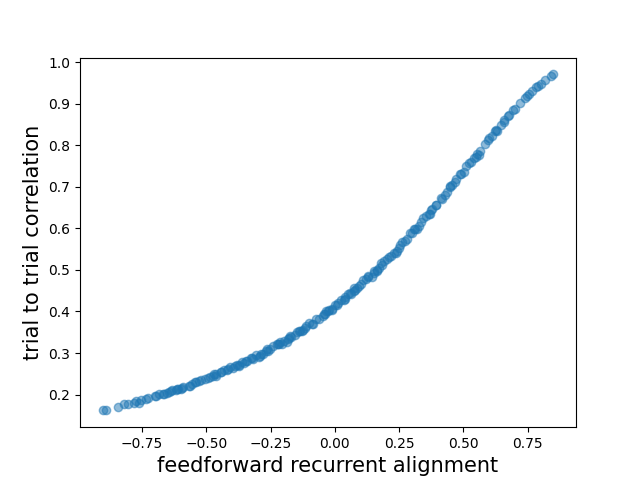
\includegraphics[width=0.5\textwidth]{../figures/ttc_sym.png}
			\label{fig:ttc_ffrec_sym}
		\end{SCfigure}
	
	We considered visually naive cortex as feedforward recurrent alignment equals zero, which could be interpreted as responses evoked by random inputs. The trial-to-trial correlation with random inputs is then smaller than the case, when the feedforward recurrent alignment takes the maximal value under inputs aligned with $\mathbf{e}_{\text{max}}$. This coincides with the experimental observations od responses from visually naive and experienced primary visual cortex of ferrets \cite{tragenap2023nature}. 
	
	Moreover, the modulation suggests a positive correlation between the feedforward recurrent alignment and the trial-to-trial correlation over the whole alignment range. The result confirms the idea that with the feedforward inputs more and more aligned with the dominant eigenvector of recurrent network, the stability between trials increases also simultaneously and almost continuously. The process of reaching higher trial-to-trial stability is therefore a process of becoming more aligned with the dominant eigenvector. 
	
	%The positive correlation between the feedforward recurrent alignment and the trial-to-trial correlation coincident with the experimental observations od responses from visually naive and experienced primary cortex of ferrets \cite{tragenap2023nature}. Moreover, the modulation suggests that 
	
	\subsubsection{Intra-Trial Stability increases with larger Alignment}
	
	Now we want to see if our modeling could capture the change in intra-trial stability during the development observed in the primary visual cortex of ferrets \cite{tragenap2023nature}. The intra-trial stability increased after the eye opening and a couple of days. The feedforward recurrent alignment hypothesis suggests that the visual experienced cortex should have a better alignment between feedforward inputs and the dominant modes in recurrent network. To confirm this idea, we would expect the intra-trial stability would be larger with better alignment between input and the dominant eigenvector. 
	
	Analogous to trial-to-trial correlation, the eigenvectors are sorted in the descending order according to the eigenvalues (\ref{eq:ascending_order}). The intra-trial stability is calculated with (\ref{eq:its_sym}).
	\vspace{-0.4cm}
	\begin{SCfigure}[0.9][h] 
		\centering
		\caption{\textbf{Correlation between feedforward recurrent alignment and intra-trial stability.} Inputs aligned to eigenvectors $\mathbf{e}_i$ of interaction matrix $J$ in the ascending order of eigenvalues (\ref{eq:ascending_order}), resulting the feedforward recurrent alignment varies approximately between $\lambda_{\text{min}}$ and $\lambda_{\text{max}}$. For each input alignment to an eigenvector, the intra-trial stability is calculated with the evoked steady state response.}
		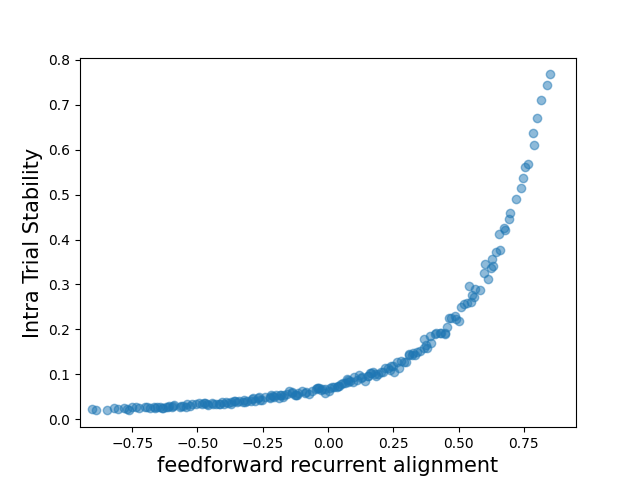
\includegraphics[width=0.5\textwidth]{../figures/its_sym.png}
		\label{fig:its_ffrec_sym}
	\end{SCfigure}

	The result (figure \ref{fig:its_ffrec_sym}) indicates also a positive correlation between the feedforward recurrent alignment and the intra-trial stability. With random feedforward inputs, the feedforward recurrent alignment take the value near zero. So the eye opening happens somewhere between feedforward recurrent equals zero and reaches maximal. Thus, before the eye opening, there is already certain alignment that lead to a certain degree of intra-trial correlation. 
	
	Furthermore, the correlation is almost exponential. So, the enhancement of the input alignment to the dominant eigenvector is more rapid after the eye opening than before the eye opening. One assumption for this phenomenon could be that after the eye opening, the environment provides more training data for the network so that the alignment between inputs and dominant eigenvector could be improved more efficiently. As a result, the responses get more intense and drive a better alignment forward. A positive loop could arise and speed up until the optimum is reached. 
	
	\subsubsection{Dimensionality decreases with larger Alignment}
	
	Dimensionality is a generally important property of neural representations and could help to understand processes for example in learning and controlling \cite{bartolo2020dimensionality, badre2021dimensionality}. A low dimensional representation will encode a diverse range of inputs into a small set of common, orthogonal activity patterns. In other words, low dimensional activity pattern require small number of basis vectors from the response space to represent itself. On the other hand, a high dimensional representation will separate even similar inputs into orthogonal activity patterns. Compare to low dimensional representation, a high dimensional activity pattern represents with a large set of basis vectors \cite{badre2021dimensionality}. 
	
	Therefore, we also aim to take a look at the change of dimensionality during the increase of alignment in the modeling. In ferrets primary visual cortex, the dimensionality decreased from days before eye opening to eye opening and then to days after eye opening \cite{tragenap2023nature}. We would then expect that the model should also suggest a decrease of dimensionality with increase of alignment between inputs and dominant eigenvector of recurrent network. 
	
	For a certain alignment, the principal component analysis reflects actually directly the dimensionality of the evoked activity pattern under this alignment. Because the principal components are the eigenvectors of response covariance, they also build up a set of basis vector for the activity pattern space. The variance ratio of principal components reflect the weight that each eigenvector takes to represent the activity pattern. Thus, if only a small number of principal components contributes the most, the activity pattern is then low dimensional. While if a broad set of principal components are similarly important, the activity pattern is high dimensional.  
	
	With the idea of earning the linear dimensionality defined as participation ratio based on the principal component analysis, the eigenvectors here are ordered in descending order, in the opposite order of ascending order defined above (\ref{eq:ascending_order}). That is 
		\begin{equation} \label{eq:descding_order}
			\mathbf{e}_{\text{max}}, ..., \mathbf{e}_i, \mathbf{e}_j, ..., \mathbf{e}_{\text{min}} \, \, \text{such that} \, \, \lambda_{\text{max}} > ...> \lambda_i > \lambda_j > ... > \lambda_{\text{min}} \, .
		\end{equation}
	%For the calculation of the linear dimensionality (\ref{eq:dim_analytical_sym}) and (\ref{eq:dim_empirical_sym}), 
	For the generation of inputs with covariance matrix $\mathbf{\Sigma^{\text{Dim}}}$ (\ref{eq:Sigma_dim}), a subset of eigenvectors $\{\mathbf{e}_i\}_{i = L, ..., L+M}$ will be chosen for $L=1, ..., \frac{n}{2}$. $M$ then determines how many eigenvectors will contribute to generate inputs and evoked activity. In each such subset of eigenvectors, the leading eigenvector is $\mathbf{e}_L$. Approximate here the feedforward recurrent alignment with the leading eigenvector only. Since $L$ is considered only in range of the first half of eigenvectors ordered as (\ref{eq:descding_order}), the range of feedforward recurrent alignment is between around $0$ and $\lambda_{\text{max}}$. The linear dimensionality analytically and empirically will be calculated according to (\ref{eq:dim_analytical_sym}) and (\ref{eq:dim_empirical_sym}). 
	
		\begin{figure}[H] 
			\centering
			\begin{subfigure}[b]{0.45\textwidth} 
				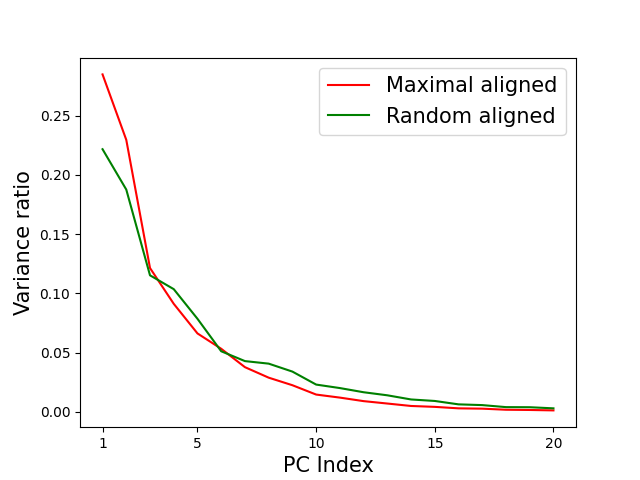
\includegraphics[width=\textwidth]{../figures/dim_align_rand_sym.png}
				\caption{}
			\end{subfigure}
			\begin{subfigure}[b]{0.45\textwidth}
				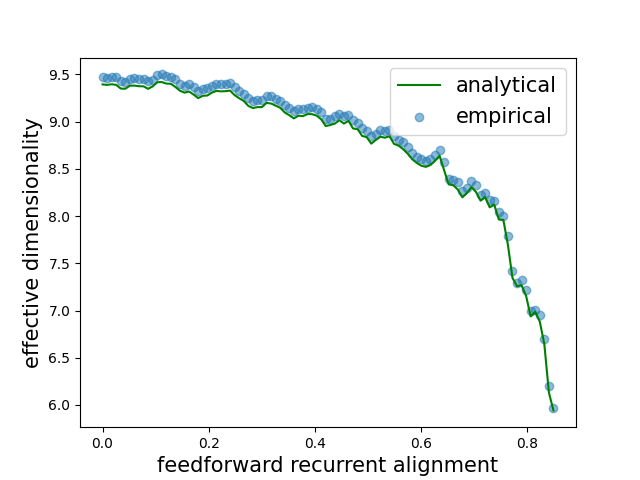
\includegraphics[width=\textwidth]{../figures/dim_sym.png}
				\caption{}
				\label{fig:dim_sym}
			\end{subfigure}
			\vspace{-0.2cm}
			\caption{\textbf{The correlation between dimensionality and feedforward recurrent alignment.} Prior experimental observation suggests that the dimensionality decreases from prior to post eye opening \cite{tragenap2023nature}. With the feedforward recurrent alignment hypothesis, dimensionality property of the neural representation could be captured. \textbf{(a)} Principal component analysis for the evoked activity under best alignment between inputs and dominant eigenvector and spontaneous random alignment. Red line for maximal alignment and green line for spontaneous alignment. \text{(b)} Achieve the correlation between dimensionality and feedforward recurrent alignment with analytical (\ref{eq:dim_analytical_sym}) and empirically (\ref{eq:dim_empirical_sym}). The green line displays the analytical approximation for dimensionality and the blue dots for empirical approximation.} 
			\label{fig:correlation_dim_ffrec_sym}
		\end{figure}
	\vspace{-0.2cm}
	As explained above, the principal component analysis helps to decode the dimensionality. The curve in figure \ref{fig:correlation_dim_ffrec_sym} (a) of the variance ratio reflects the dimensionality. Spontaneous random alignment has a flatter variance ratio curve, indicating a broader range of eigenvector contribution. Therefore, the spontaneous random alignment has a higher dimensionality. With the feedforward recurrent alignment hypothesis, the spontaneous random alignment matches the state before the eye opening and the maximal alignment for the state after eye opening. Therefore, the hypothesis results the same tendency of dimensionality decrease that observed in ferrets\cite{tragenap2023nature}.
	
	In total, a negative correlation between the dimensionality and feedforward recurrent alignment is shown in figure \ref{fig:correlation_dim_ffrec_sym} (b). The correlation forms nearly a flipped logarithmic function. The error between analytical and empirical results are small, which confirmed the well approximation formulated analytically by (\ref{eq:dim_analytical_sym}). 
	
	Besides, the flipped logarithmic correlation suggests the similar principle for intra-trial stability (figure \ref{fig:its_ffrec_sym}). After eye opening, the reduction of dimensionality becomes larger when the feedforward inputs aligns better with dominant eigenvector. It could be the case, that after the eye opening, the recurrent network tries to encode the environment information with large number of eigenvectors, which is costing for the system. After a period of time of getting used to the stimuli, the system speed up to find out a more efficient encoding with fewer eigenvectors and the information becomes more determined. 
	%After finding out a better solution, the improvement will be speed up until the optimum encoding with at least number of eigenvectors. 
	
	\subsubsection{Alignment to spontaneous activity increases with larger Alignment}
	
	Spontaneous activity in neural systems is defined as neural activity that is not driven by an external stimulus. The activity patterns of spontaneous activity is not completely random and have often unique spatiotemporal patterns that instruct neural circuit development in the developing brain. Moreover, normal and aberrant patterns of spontaneous activity underline behavioral states and diseased conditions in adult brains. Therefore, the spontaneous activity is essential for the understanding of brain development \cite{imaizumi2018spontaneous}. The alignment between activity pattern and spontaneous activity pattern could show the structural relation between patterns. Besides, it could also reflect the presentation of spontaneous activity in other activity patterns. 
	
	In baby ferrets' brain, a transformation from visual responses that are loosely aligned with spontaneous activity in the cortex before eye opening to the reliable and well aligned responses several days after eye opening were observed \cite{tragenap2023nature}. Thus, we will expect that the feedforward recurrent hypothesis can reflect the tendency that evoked activity aligned better to spontaneous activity during the development of brain. 
	\vspace{-0.4cm}
		\begin{figure}[H] 
			\centering
			\begin{subfigure}[b]{0.45\textwidth} 
				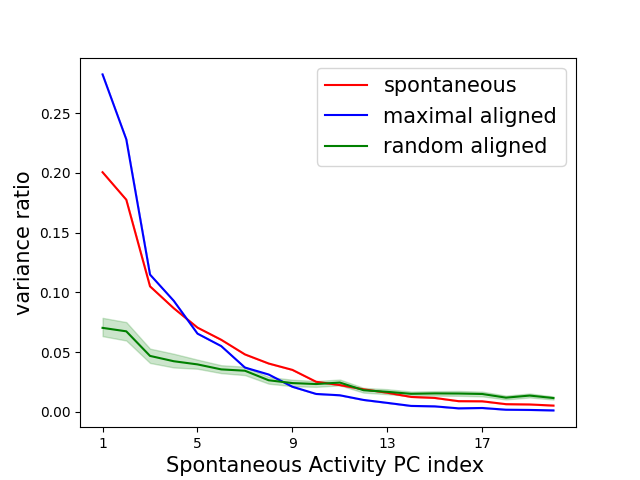
\includegraphics[width=\textwidth]{../figures/align_to_spont_act_variance_ratio.png}
				\caption{}
				\label{fig:variance_ratio_sym}
			\end{subfigure}
			\begin{subfigure}[b]{0.45\textwidth}
				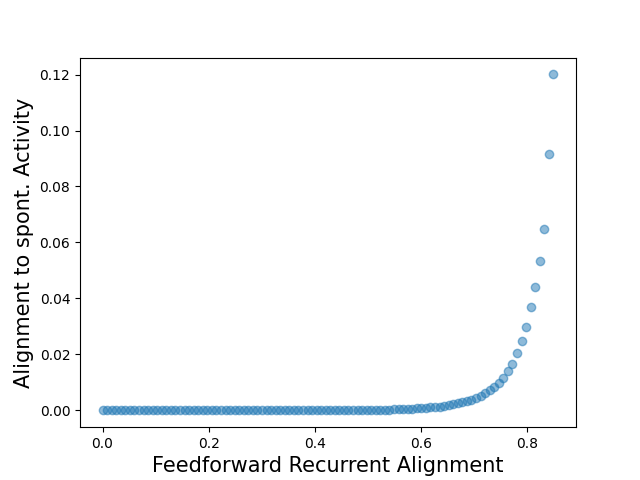
\includegraphics[width=\textwidth]{../figures/spont_align_ffrec_sym.png}
				\caption{}
				\label{fig:align_spont_sym}
			\end{subfigure}
			%\vspace{-0.1cm}
			\caption{\textbf{Correlation between alignment to spontaneous activity and feedforward recurrent alignment.} Spontaneous activity reflects inputs from wide range of different sources and considered to already aligned to the recurrent network\cite{tragenap2023nature}. Aligning activity patterns to spontaneous activity is in principle to explain the activity pattern by the principal components of spontaneous activity. \textbf{(a)} Variance ratio (\ref{eq:var_explain_spont_act_sym}) of spontaneous activity, evoked activity by feedforward input maximally aligning to recurrent network, and evoked activity by randomly aligning to recurrent network explained by principal components of spontaneous activity. The red line illustrates the variance ratio of spontaneous activity, blue line the maximal alignment, and green line the random alignment. Shadow shows the 95\% confident interval for 50 networks. \text{(b)} The correlation between final alignment score to spontaneous activity and feedforward recurrent alignment better than random alignment calculated with (\ref{eq:align_to_spont_act_sym}). The eigenvalues are ordered in the same way as (\ref{eq:descding_order}). Only the first half eigenvectors are taken into account to determine the correlation.}
			\label{fig:align_spont_act_sym}
		\end{figure}
	
	Under the assumption that at eye opening, the patterns of feedforward inputs are not as well aligned to the recurrent network as the spontaneous activity, the evoked and spontaneous pattern overlaps only little (figure \ref{fig:align_spont_act_sym}(a), visually comparing green line to red line.) It could be observed here that only the last few principal components has the similar variance ratio, while the first few dominant eigenvectors differs a lot. On the contrary, experience-driven changes that optimize the feedforward-recurrent alignment results in a stronger overlap between distributions of evoked and spontaneous activity pattern (figure \ref{fig:align_spont_act_sym}(a), visually comparing red line to blue line.). Most of the principal components has the similar explained variance ratio. In both cases, the hypothesis matches experimental observations in baby ferrets' brain \cite{tragenap2023nature}.
	
	To visualize and quantify the overlap between activity patterns from evoked and endogenous pattern, we considered the summarized alignment score (\ref{fig:align_spont_act_sym}). A exponential correlation between alignment to spontaneous activity and feedforward recurrent alignment (figure \ref{fig:align_spont_act_sym}(b)) is suggested by the modeling. The strong growth of overlaps between evoked and endogenous activity starts only shortly before the optimal experience-driven alignment, indicating that the alignment could require a large amount of experience and training. The costly process to optimal alignment to spontaneous activity could on the other hand reflect the importance of the connection between evoked and endogenous activity patterns. 
	
	\clearpage
	\subsection{Evaluation of Feedforward Recurrent Alignment Modulations for asymmetric Recurrent Interaction Networks} \label{sec:asymmetric_results}
	For symmetric interaction networks, the feedforward recurrent alignment hypothesis and the modulation based on it can demonstrate the response properties observed in ferrets \cite{tragenap2023nature} (section \ref{sec:results_symmetric}). With better alignment between inputs and recurrent network, key results of the response properties were
		\begin{itemize}
			\item The trial-to-trial correlation increases.
			\item The intra-trial stability increases.
			\item The Dimensionality decreases.
			\item The Alignment of evoked activity to spontaneous activity increases.
		\end{itemize}
	
	However, since the symmetric interaction matrices simplify the neural connection dramatically, we try to embed the more biological realistic asymmetric interaction matrices. Considering the modifications listed in methods (section \ref{sec:modify_ffrec_alignment_score}), we want to evaluate the results based on the key results we got with symmetric interaction matrices. 
	
	Firstly, we check if the feedforward recurrent alignment score keeps the proportionality to eigenvalues as shown with (\ref{eq:ffrec_equals_eigval}). We expect that a suitable modification could keep the positive correlation with eigenvalues. Then, we go through the four response properties to verify if the tendency above are still kept with increased alignment between inputs and recurrent network. 
	
	\subsubsection{Monotony of Feedforward Recurrent Alignment Score in dependence of Eigenvalues}
	
	During the development, suggested by feedforward recurrent alignment hypothesis for symmetric interactions, the inputs align from eigenvectors with small eigenvalues to eigenvectors with large eigenvalues. Due to the formulation (\ref{eq:ffrec_align}), feedforward recurrent alignment is proportional to the corresponding eigenvalue of the eigenvector that is aligned with input (\ref{eq:ffrec_equals_eigval}). 
	
	When considering the asymmetric interaction network, keeping the hypothesis that the input align more and more to the eigenvector with maximal eigenvalue, we examine if the modified feedforward recurrent alignment score could still keep the proportionality that the modified variations increase with larger eigenvalues.
	%\footnote{Order the complex eigenvalues of the asymmetric interaction matrix through comparing the real parts. Undertaken this comparison with Python build-in function }. 
	If the positive correlation between the feedforward recurrent alignment and eigenvalues could be kept, the alignment score could at least quantify how well input align to the dominant eigenvector and thus quantify the alignment between input and recurrent network. 
	
	% figure of proportionality 
%		\begin{figure}
%			\centering
%			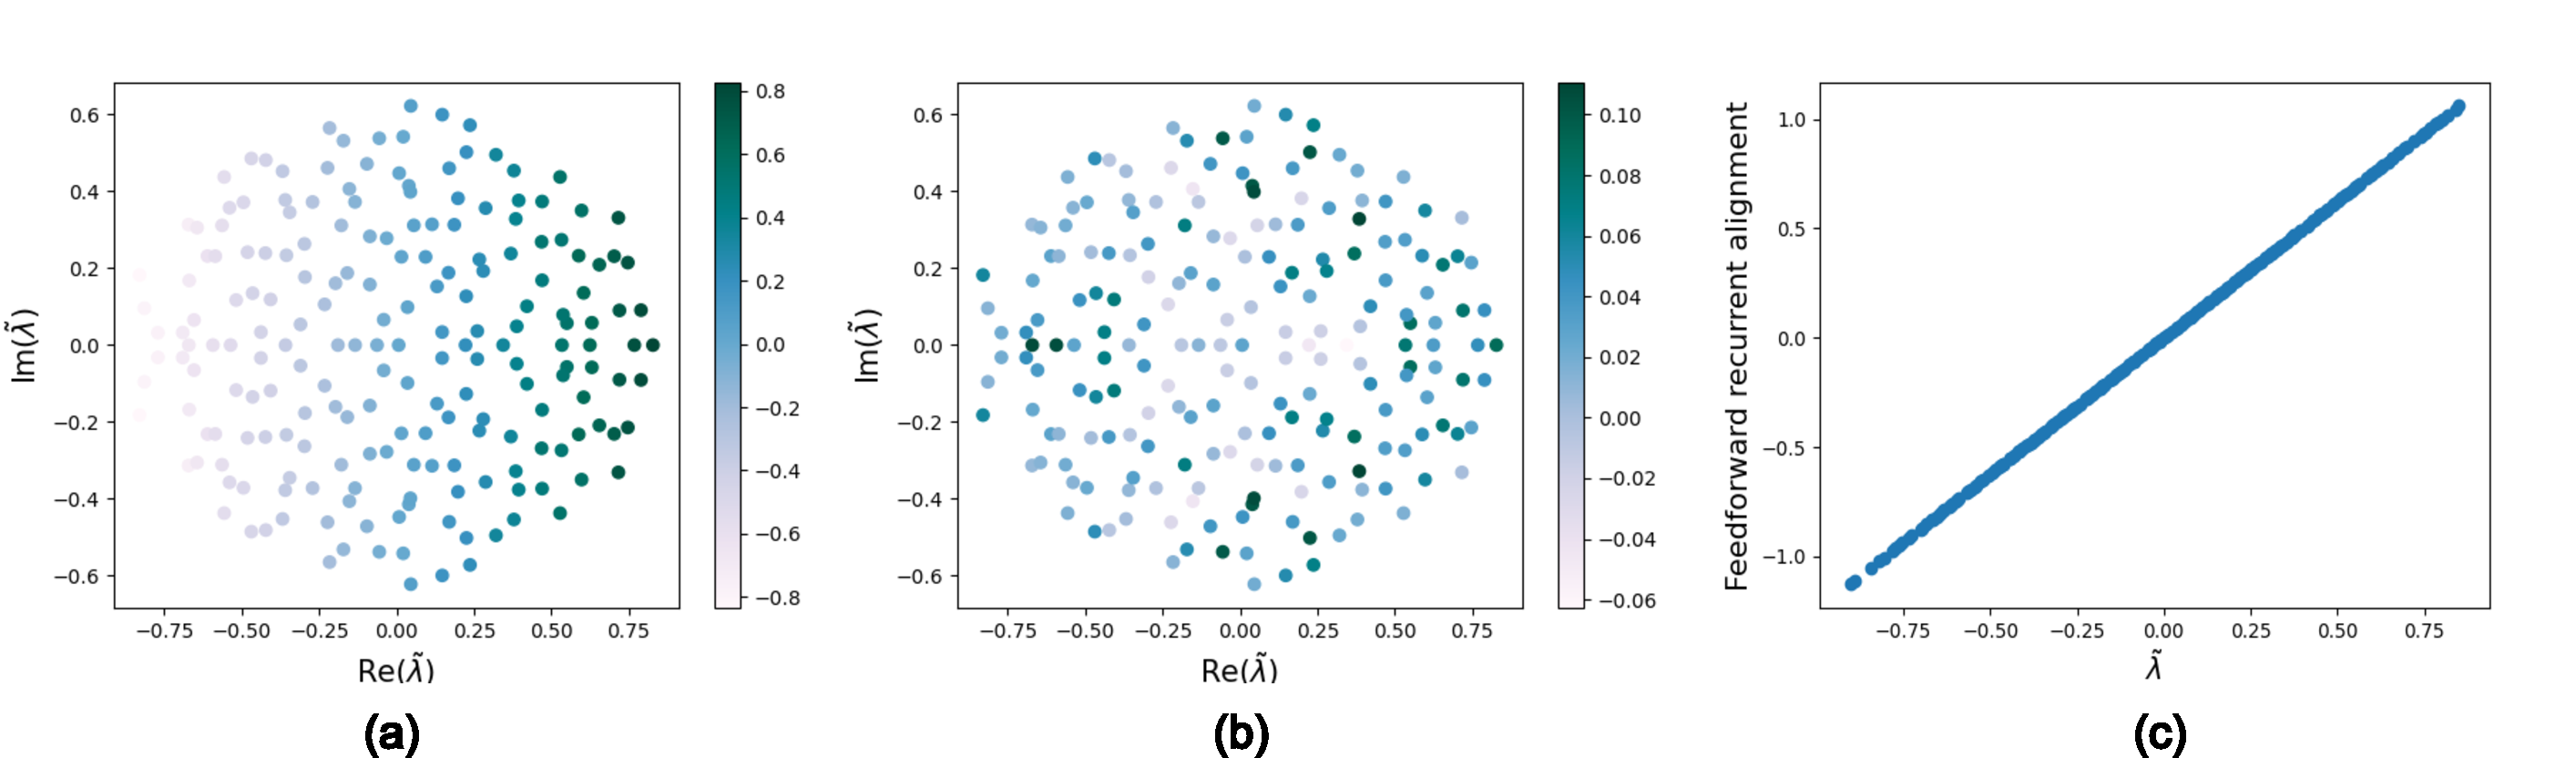
\includegraphics[width=\textwidth]{../figures/ffrec_eigval_proportion.pdf}
%			\caption{text}
%		\end{figure}
		\begin{figure}
			\centering
			\begin{subfigure}[b]{0.4\textwidth}
				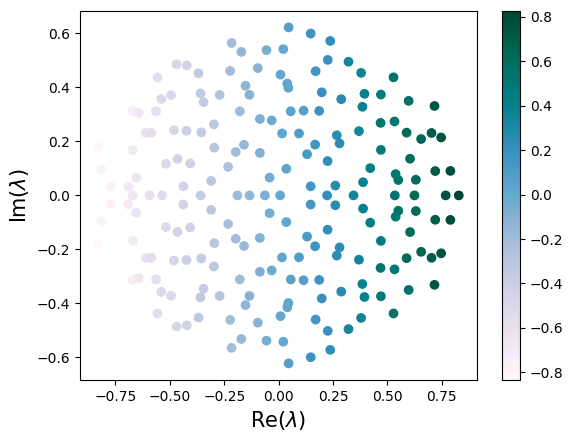
\includegraphics[width=\textwidth]{../figures/ffrec_eigval_real_part.png}
				\caption{}
				\label{fig:ffrec_real_part}
			\end{subfigure}
			\begin{subfigure}[b]{0.425\textwidth}
				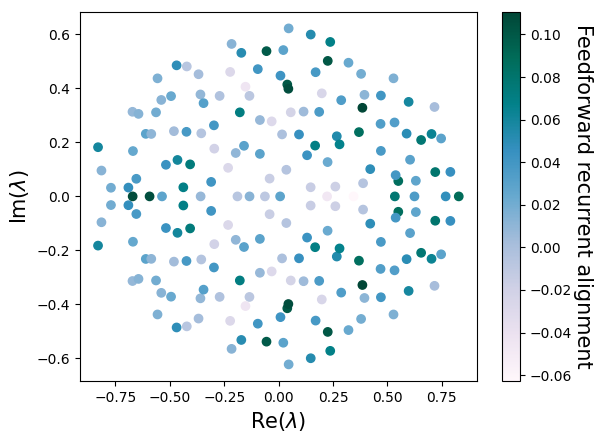
\includegraphics[width=\textwidth]{../figures/ffrec_eigval_mag.png}
				\caption{}
				\label{fig:ffrec_mag}
			\end{subfigure}
%			\begin{subfigure}[b]{0.3\textwidth}
%				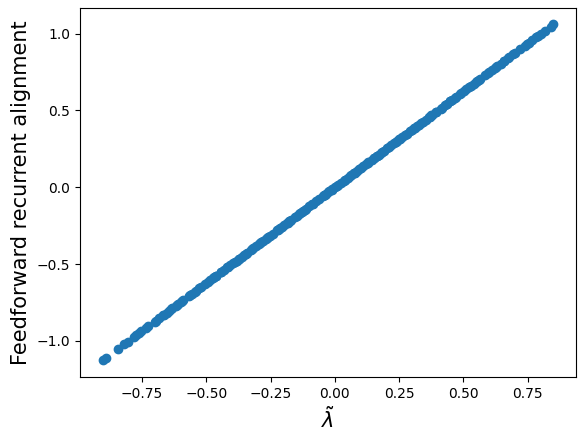
\includegraphics[width=\textwidth]{../figures/ffrec_eigval_symmetrized_J.png}
%				\caption{}
%			\end{subfigure}
			\caption{\textbf{Correlation between eigenvalues and feedforward recurrent alignment.} To verify the considered modifications, a positive correlation between eigenvalues and feedforward recurrent alignment is advantageous. Represent the correlation in the complex plane, since eigenvalues are complex. Color bar indicate the size of feedforward recurrent alignment. The darker the color, the larger the alignment score.  \textbf{(a)} Representation of alignment score calculated with modification \ref{sec:modicication_real_part} (\ref{eq:ffrec_real_part}) in complex plane. \textbf{(b)} Representation of alignment score calculated with modification \ref{sec:modification_magnitude} (\ref{eq:ffrec_mag}) in complex plane.}
		\end{figure}
	
	% Conclusion and mathematical explanation of Results for the proportionality.
	\paragraph{Modification 1}: Apply the real part of complex inputs (\ref{eq:ffrec_real_part}).
	
	With the feedforward recurrent alignment, we mainly consider the correlation of alignment score and eigenvalues under alignment between inputs and eigenvectors of recurrent network $J$. Inserting inputs equal the eigenvectors $h = e_i \in \mathbb{C}^{n \times 1}$ into (\ref{eq:ffrec_real_part}), it leads to
		\begin{equation}
			\nu_{\text{Re}} = \frac{\text{Re}(e_i)^T J \text{Re}(e_i)}{\Vert \text{Re}(e_i)\Vert^2} \, .
		\end{equation}
	Because $\Vert e_i \Vert = c \Vert \text{Re}(e_i) \Vert$ with $c \in \mathbb{R_{+}}$ a general positive constant, we could get the proportionality between alignment score and the real part of eigenvalues $\text{Re}(\lambda_i)$ of $J$ :
		\begin{equation}
			\begin{split}
				\nu_{\text{Re}} & = c \text{Re}\left( \frac{e_i}{\Vert e_i \Vert} \right)^T J \, \text{Re}\left( \frac{e_i}{\Vert e_i \Vert} \right) \\
				& = c \text{Re} \left( \frac{e_i^T}{\Vert e_i \Vert} J \frac{e_i}{\Vert e_i \Vert} \right) \\
				& = c \text{Re}(\lambda_i) \, ,
			\end{split}
		\end{equation}
	with $c$ general positive constant.
	
	The positive correlation between alignment and real part of eigenvalues $\lambda_i$ could also be observed in representation in complex plane (figure \ref{fig:ffrec_real_part}). With increasing real part of eigenvalue, the size of alignment score also becomes larger. Furthermore, there is no correlation found in the direction of imaginary part of eigenvalues, since the alignment score only depends on the real part. 
	
	\paragraph{Modification 2}: Apply the magnitude for each neuron input (\ref{eq:ffrec_mag}).
	
	When the inputs are aligned to eigenvectors $e$ of $J$, the feedforward recurrent alignment could be expressed with $\vert e \vert := (\vert e_{i} \vert)_{i = 1, ..., n} \in \mathbb{C}^{n \times 1}$ after inserting into (\ref{eq:ffrec_mag}). As the euclidean norm of vector $\vert e \vert$ is the same as the norm directly on the complex eigenvector $\Vert e \Vert_2$, the final feedforward recurrent alignment score can be then formulated as following:
		\begin{equation}
			\begin{split}
				\nu_{\text{mag}} & = \frac{\vert e \vert^T J \vert e \vert}{\Vert e \Vert^2} \\
			%	& = \frac{\sum_{j=1}^{n} \sqrt{x_j^2 + y_j^2} \left( \sum_{i = 1}^{n} \sqrt{x_i^2 + y_i^2} J_ij \right)}{\sum_{i=1}^{n}}
				& = \frac{\sum_{j=1}^{n} \vert e_{j} \vert \left( \sum_{i = 1}^{n} \vert e_{i} \vert J_{ij} \right)}{\Vert e \Vert^2} \, ,
			\end{split}
		\end{equation}
	where $e_i, e_j$ are the $i$-th and $j$-th element of the vector $e$, and $J_{ij}$ the matrix element at $i$-th row and $j$-th column. 
	
	Therefore, no direct correlation between the alignment score and eigenvalues $\lambda$ can be established. The lack of correlation is also represented in the complex plane (figure \ref{fig:ffrec_mag}). 
	
	\paragraph{Modification 3}: Align the inputs to eigenvectors of symmetrized network (\ref{eq:ffrec_symmetrized}).
	
	Instead of aligning the inputs to eigenvectors of original asymmetric recurrent network and thinking about modifications of eigenvectors to calculate the feedforward recurrent alignment score, we now directly align the inputs to real eigenvectors $\tilde{e}$ of symmetrized recurrent network $\tilde{J}$ as an approximation. However, the alignment score is projected to the original asymmetric recurrent network (\ref{eq:ffrec_symmetrized}). There is still a proportionality between the eigenvalues of symmetrized network and alignment score. 
	
		\begin{SCfigure}[0.95][h] 
			\centering
			\caption{\textbf{Positive correlation between feedforward recurrent alignment score and eigenvalues of symmetrized network.} Project the inputs to the eigenvectors of symmetrized network to refer the development instead of the projection to the original asymmetric network. The correlation between the alignment score (y-axis) based on the original recurrent network to the eigenvalues of symmetrized network (x-axis) remains positive.}
			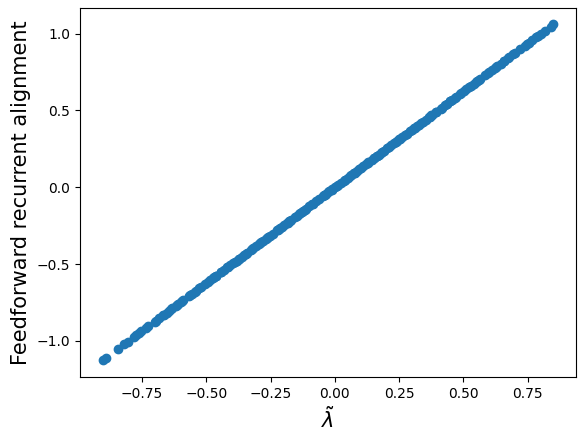
\includegraphics[width=0.45\textwidth]{../figures/ffrec_eigval_symmetrized_J.png}
			\label{fig:ffrec_symmetrized}
		\end{SCfigure}
	Since the symmetrized recurrent network $\tilde{J}$ is received by (\ref{eq:symmetrized_J}), the proportionality shown in figure \ref{fig:ffrec_symmetrized} can be obtained as the following:
		\begin{equation}
			\begin{split}
				&\frac{\tilde{e}^T \tilde{J} \tilde{e}}{\Vert \tilde{e} \Vert^2} = \frac{\tilde{e}^T \frac{J + J^T}{2} \tilde{e}}{\Vert \tilde{e} \Vert^2} = \frac{1}{2} \left( \frac{\tilde{e}^T J \tilde{e}}{\Vert \tilde{e} \Vert^2} + \frac{\tilde{e}^T J^T \tilde{e}}{\Vert \tilde{e} \Vert^2} \right) \\
				\Rightarrow \,  & 2 \frac{\tilde{e}^T \tilde{J} \tilde{e}}{\Vert \tilde{e} \Vert^2} - \frac{\tilde{e}^T J^T \tilde{e}}{\Vert \tilde{e} \Vert^2} = \frac{\tilde{e}^T J \tilde{e}}{\Vert \tilde{e} \Vert^2} \\
				\Rightarrow \, & 2 \tilde{\lambda} - c = \frac{\tilde{e}^T J \tilde{e}}{\Vert \tilde{e} \Vert^2} \text{ with } c := \frac{\tilde{e}^T J^T \tilde{e}}{\Vert \tilde{e} \Vert^2} \in \mathbb{R} \text{ and $\tilde{\lambda}$ the corresponding eigenvalue of $\tilde{e}$} \\
				\Rightarrow \, & \frac{\tilde{e}^T J \tilde{e}}{\Vert \tilde{e} \Vert^2} \propto \tilde{\lambda} \, .
			\end{split}
		\end{equation}
	
	\paragraph{Conclusion} After the analysis above for all modifications, our expectation of contained positive correlation are kept when considering the real part (modification 1) and alignment with symmetrized recurrent network (modification 3). The variant with magnitude (modification 2) fails to fulfill the correlation. Thus, we will leave the modification 2 out without further analysis for response properties in the following section. 
	
	\subsubsection{Representing Response Properties with modified Feedforward Recurrent Alignment} \label{sec:asym_ffrec_response}
	
	After verifying the expected correlation between feedforward recurrent alignment score and the network that the inputs are aligned to, we will check out if the remaining modifications could still reflect the four experimental observations listed at the beginning of the section \ref{sec:asymmetric_results} with remaining modification 1 and 3. 
	\begin{itemize}
		\item When aligning the inputs to the asymmetirc recurrent network to test the feedforward recurrent alignment hypothesis, the modification 1 considers the complex input only with real part of eigenvectors. 
		\item The modification 3 aligns the inputs to symmetrized recurrent network but calculate the alignment score still with original asymmetric network. 
	\end{itemize}
	
	Besides, since the asymmetirc recurrent network is constructed with certain degree of symmetry (\ref{eq:asym_interaction_matrix}), we also controlled how much the degree of symmetry influences the results. 
	
	\paragraph{Trial-to-trial Correlation}
	
	Trial-to-trial correlation is the averaged correlations between trials (\ref{eq:ttc_sym}). The expectation is a positive correlation between feedforward recurrent alignment and trial-to-trial correlation, independent of the degree of symmetry. 
		\begin{figure}[H]
			\centering
			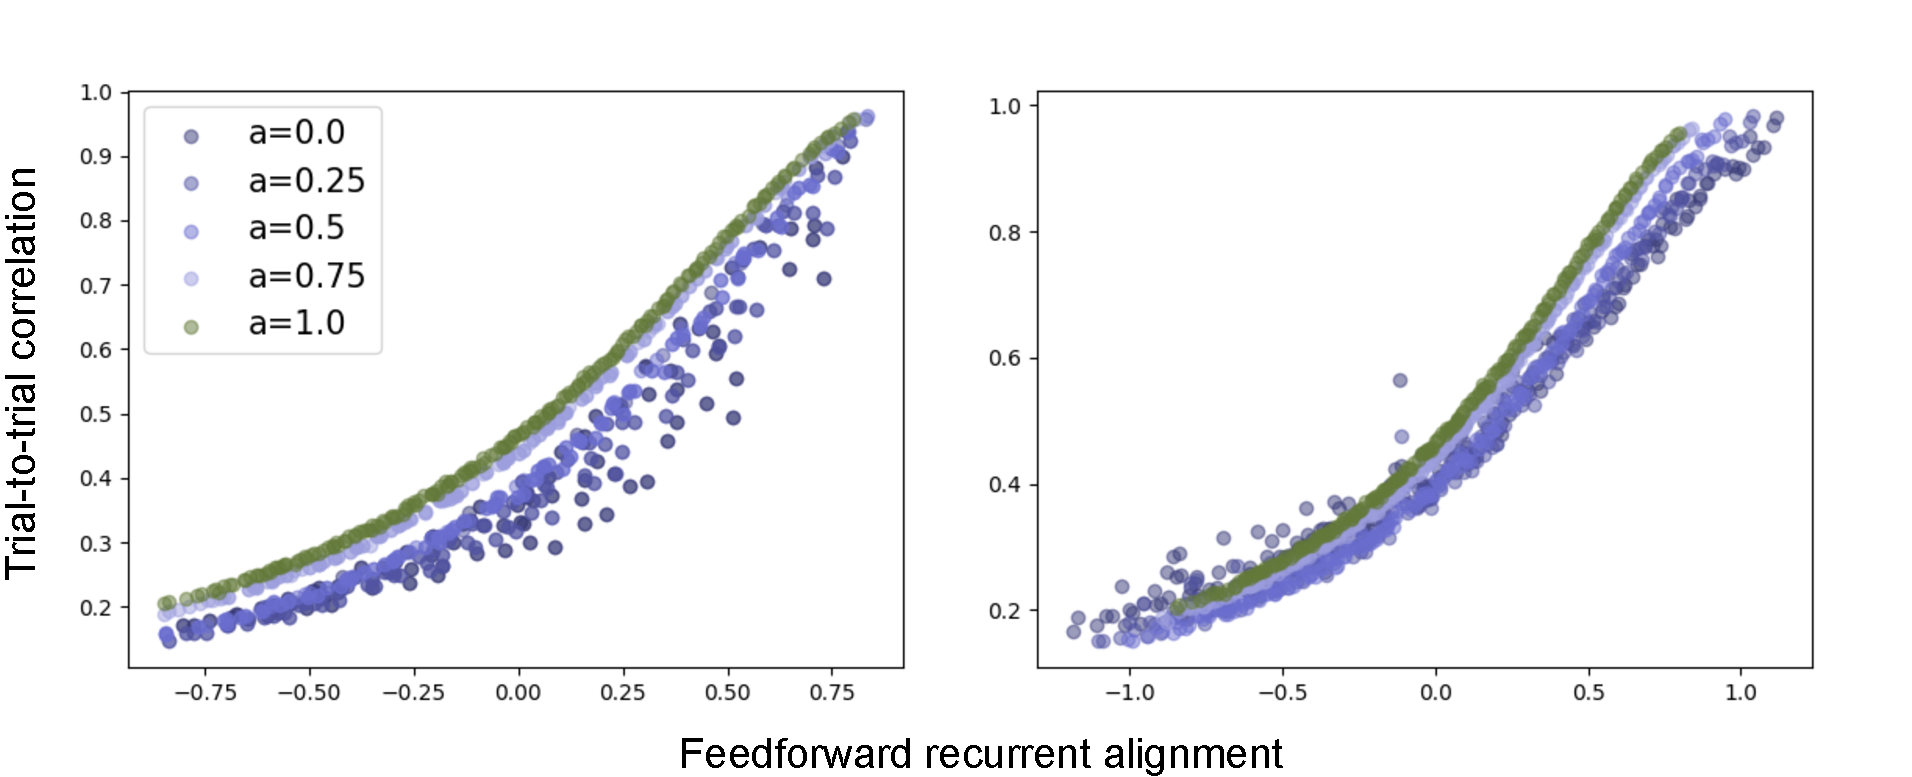
\includegraphics[width = \textwidth]{../figures/ttc_asym.pdf}
			\caption{\textbf{Correlation between trial-to-trial correlation and feedforward recurrent alignment with asymmetric recurrent network inclusive the influence of symmetry.} For different degree of symmetry $a$, different color dots are applied shown in legend. The green color with $a=1.0$ illustrates the case of symmetric network. The most dark purple $a=0.0$ represents the asymmetric network without any influence of symmetry. The x-axis shows the alignment score calculated with considered modifications and the y-axis indicates the trial-to-trial correlation calculated with aligned inputs through (\ref{eq:ttc_sym}) \textbf{Left}: Result generated with modification 1 (only consider real part). \textbf{Right}: Result with modification 3 (symmetrized recurrent network).}
			\label{fig:ttc_asym}
		\end{figure}
	The results (figure \ref{fig:ttc_asym}) point out that the trendy of positive correlation keeps while the network increases its asymmetry for both modifications 1 and 3. 
	
	However, when the network is fully asymmetric, the correlation has larger dispersion with modification 1 (only real part). We suspect that the reason is that in the case of full asymmetry, more information got lost because of only considering information from real part of aligned inputs. If there is certain degree of symmetry, a part of information during the alignment originates from the symmetric recurrent network and therefore for this part of alignment, no information get lost while only taking the real part of aligned inputs. Aligning to fully asymmetric recurrent network and only taking real part of aligned inputs, all neurons receive as a result incomplete information. Therefore, the correlation between evoked patterns will be disturbed mostly. 
	
	In the case of modification 3 (align inputs to symmetrized network), the correlation is almost maintained over all degree of symmetry. 
	
	\paragraph{Intra-trial Stability}
	
	Intra-trial stability is the averaged time-delayed activity correlation inside one single trial. As the name indicates, it shows how stable the information is represented inside one trial. With the result from symmetric recurrent network, we expect a similar exponential positive correlation as in figure \ref{fig:its_ffrec_sym} also with the asymmetric recurrent network. The degree of symmetry should also not influence the result significantly since we assume that the hypothesis should also work well with asymmetric recurrent networks generally.
		\begin{figure}[H]
			\centering
			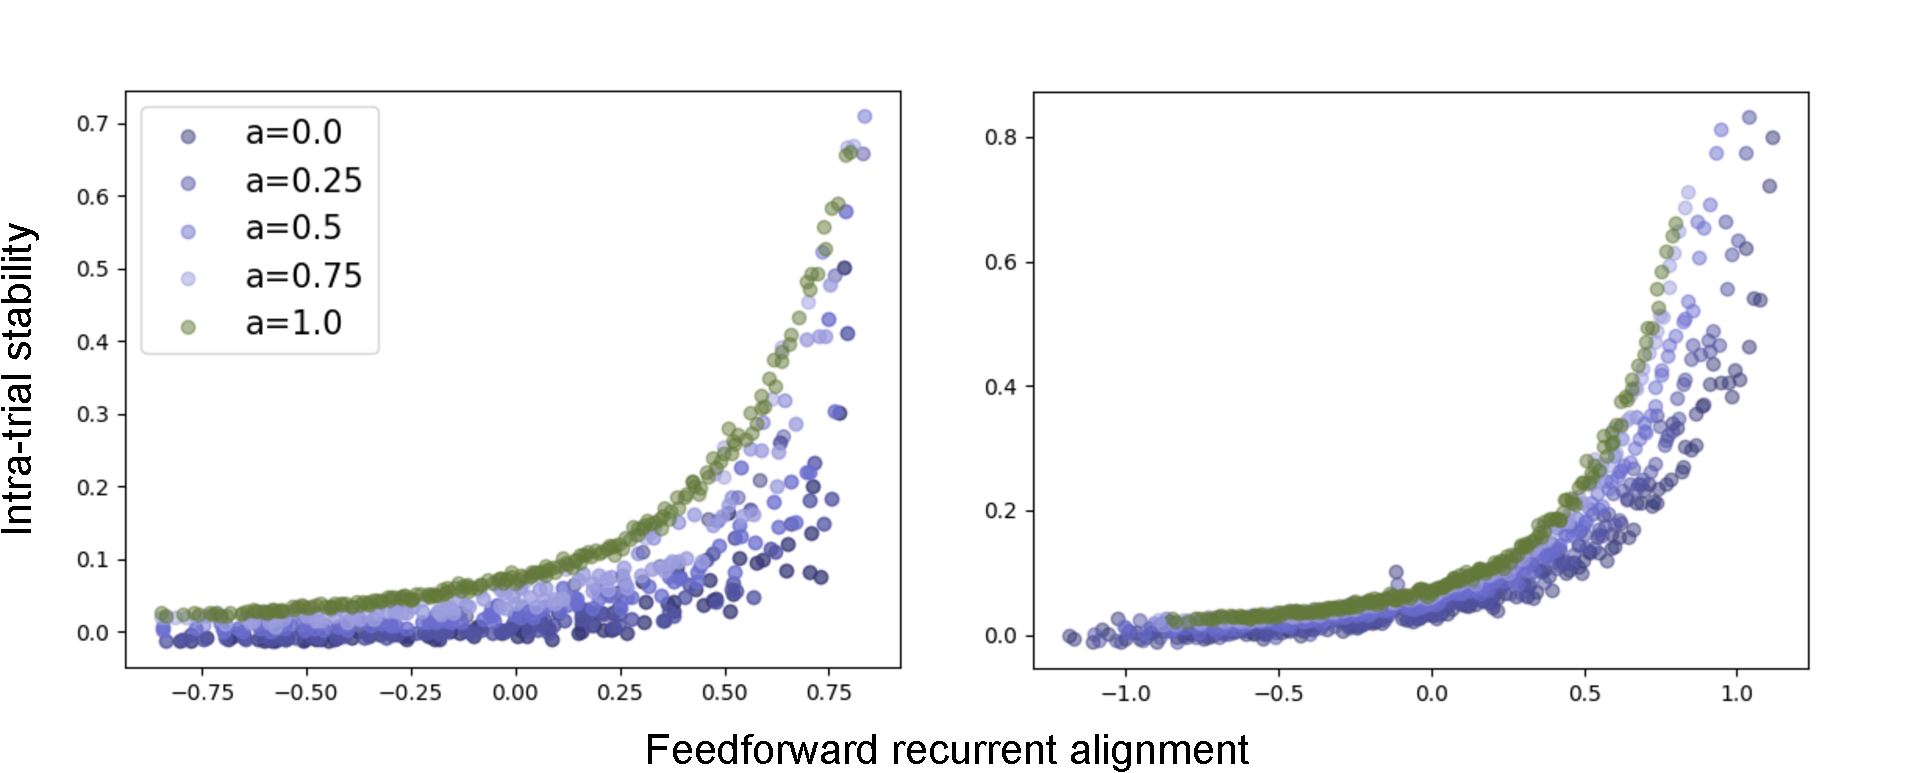
\includegraphics[width=\textwidth]{../figures/its_asym.pdf}
			\caption{\textbf{Correlation between intra-trial stability and feedforward recurrent alignment with asymmetric recurrent network considering the influence from degree of symmetry.} For multiple degrees of symmetry $a$, different color dots are applied shown in legend. From complete symmetric $a = 1.0$ (as control) to full asymmetric recurrent network, the corresponding feedforward recurrent alignment (x-axis) is plotted against the intra-trial stability (y-axis). \textbf{Left}: Result with modification 1 (only real part of aligned inputs). \textbf{Right}: Result with modification 3 (align input to symmetrized network).}
			\label{fig:its_asym}
		\end{figure}
	We suspect with the similar reason as in trial-to-trial correlation that for modification 1, the lost of imaginary part information of aligned inputs could lead to increased dispersion with larger asymmetry of network (figure \ref{fig:its_asym} left panel). 
	
	For modification 3, except for the expected exponential positive correlation between intra-trial stability and feedforward recurrent alignment score, we also observe that the dispersion is more noticeable with increased asymmetry. So, the degree of symmetry influence here more significant than in trial-to-trial correlation. Furthermore, similar to modification 1, although align inputs to the symmetrized network, the lost of information also got lost with the increased asymmetry. Imagine if having a total symmetric network, the result of symmetrization is the network itself and therefore no information is lost in eigenvectors. However, if having a fully asymmetric recurrent network, after symmetrization, information that stored in complex eigenvectors get transformed to lower dimension real eigenvectors completely. Thus, when align inputs to the symmetrized asymmetric network, transformed information could be the reason for larger dispersion. 
	
	\paragraph{Dimensionality}
	
	Dimensionality reflects the complexity of the information they encoded. A high dimensional activity pattern needs more orthogonal activity pattern for representation then a low dimensional activity pattern and thus indicates larger variability and higher complexity of contained information. Modification 1 and 3 change the eigenvectors for construction of input variance and the eigenvalues for calculation of effective dimensionality (section \ref{sec:modification_asym} eq. (\ref{eq:modifications_dim}), (\ref{eq:modification_eff_dim})). 
	
	If both modifications work well, the results should be similar to result from symmetric recurrent network (figure \ref{fig:dim_sym}). Low degree of symmetry is allowed to lead to small range of dispersion, which however should still keep the tendency of decreased dimensionality with increased alignment score. % Refer calculation in method + Expectiations
		\begin{figure} [H]
			\centering
			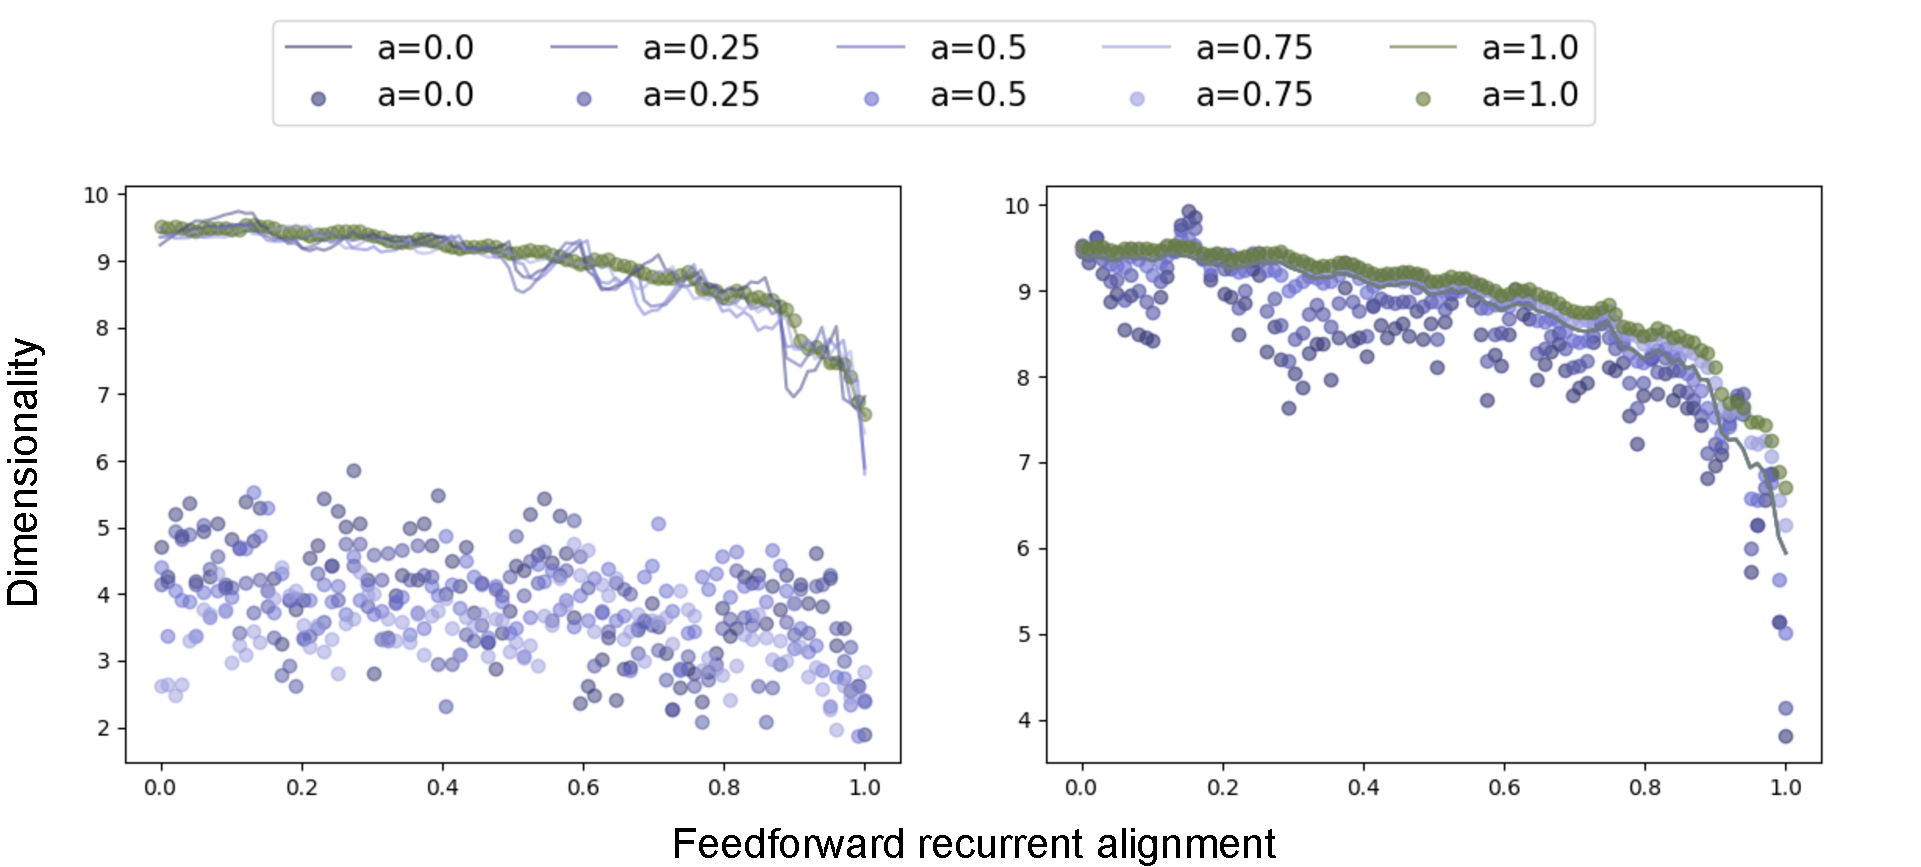
\includegraphics[width=\textwidth]{../figures/dim_asym.pdf}
			\caption{\textbf{Analytical and empirical effective dimensionality in correlation with feedforward recurrent alignment with asymmetric recurrent network. Impact on the correlation from the degree of symmetry in network.} The full symmetric recurrent network ($a = 1.0$) is control for other cases with $a < 1.0$. When $a = 0.0$, the recurrent network is fully asymmetric. The dots represents the empirical approximation for effective dimensionality (\ref{eq:dim_empirical_sym}). The lines are for the analytical calculation for dimensionality adjusted to modification 1 and 3 (section \ref{sec:modification_asym} eq. (\ref{eq:modifications_dim}), (\ref{eq:modification_eff_dim})). \textbf{Left}: Result with modification 1 (only real part of aligned inputs and eigenvalues for analytical dimensionality). \textbf{Right}: Result with modification 3 (align inputs and to symmetrized recurrent network).}
			\label{fig:dim_asym}
		\end{figure}
	% Reason for left: the analytical solution under assumption that the basis of Sigma_Dim are orthogonal-- got lost with Re(e). Therefore large difference between analytical and empirical solution. --> at this step the modification 1 is also not good. Could let out. 
	With modification 1 (figure \ref{fig:dim_asym} left panel), the empirical dimensionality differs a lot from the analytical calculation of dimensionality. Besides, there is no significant correlation between dimensionality and feedforward recurrent alignment with empirical data. The reason for that could be the lost of orthogonality between the real part of eiegenvectors, that is 
		\begin{equation}
			e_i \perp e_j  \, \, \nRightarrow \text{Re}(e_i) \perp \text{Re}(e_j) \, \, \forall i, j = 1, ..., n \, .
		\end{equation}
	As a result, the covariance matrix $\Sigma^{\text{Dim}}$ (\ref{eq:modifications_dim}) is not necessarily constructed with orthogonal vectors anymore, which contradicts the assumption of reflecting dimensionality by projecting activity pattern on orthogonal patterns that are also applied to construct covariance matrix. 
	
	With modification 3, the results fulfill largely the expectations: the negative correlation between dimensionality and feedforward recurrent alignment is kept in both analytical and empirical approximations. Little dispersion is due to the structural information lost when symmetrize the asymmetric recurrent network and align the inputs to symmetrized eigenvectors. 
	
	Thus, until this step, we would also drop the modification 1 and only further consider the modification 3. 
	
	\paragraph{Alignment to spontaneous activity}
	The alignment of evoked activity pattern to the endogenous pattern measures the overlap between their variance ratio curves explained by endogenous pattern (\ref{eq:var_explain_spont_act_sym}), for example the overlaps between curves in figure \ref{fig:variance_ratio_sym}. Only modification 3 is left for the evaluation. 
	
	Similar to prior cases, if the modification works, we expect the correlation tendency between alignment to spontaneous activity and feedforward recurrent alignment score would also be kept as with symmetric recurrent network (figure \ref{fig:align_spont_sym}). The alignment to spontaneous activity is modified with (\ref{eq:Sigma_spont_asym}) and calculate with (\ref{eq:align_to_spont_act_sym}). 
		\vspace{-0.5cm}
		\begin{SCfigure}[0.9][h] 
			\centering
			\caption{\textbf{The correlation between alignment to spontaneous activity and feedforward recurrent alignment considering influence from degree of symmetry in the recurrent network.} As control, fully symmetric recurrent network $a=1.0$ is represented with dark green dots. For different degree of symmetry from $a = 0.75$ to $0$, the darker the dot color, the more asymmetric is the recurrent network. }
			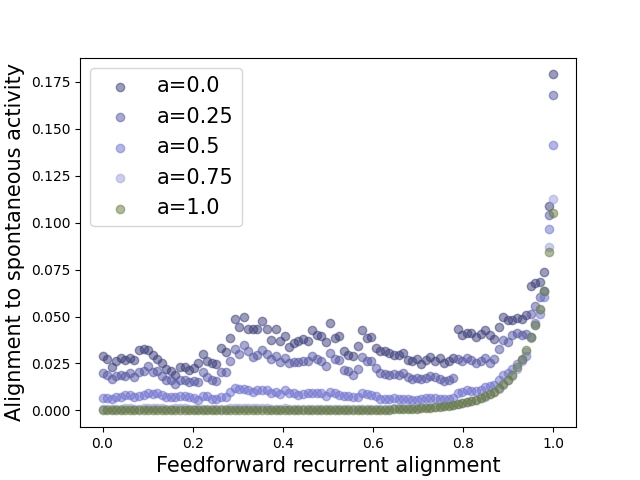
\includegraphics[width=0.5\textwidth]{../figures/align_to_spont_asym_symmetrized_rescaled.png}
			\label{fig:align_to_spont_asym}
		\end{SCfigure}
	
	The dispersion increases with the degree of asymmetry due to the increased information lost, but the general tendency that alignment of evoked activity pattern to spontaneous activity becomes larger when the alignment of inputs to symmetrized recurrent network is larger. With high degree of symmetry, e.g. $a = 0.75$, the correlation is significantly similar to it with total symmetric recurrent network.
	
	\paragraph{Conclusion}
	After evaluating the rest modifications 1 and 3 with four perspectives of response properties, the modification 1 is filtered out because of the lack of orthogonality between eigenvectors after modification. The modification 3 performs at the end the best and could generally fulfill the expectations of correlations between the response properties and feedforward recurrent alignment. 
	
	Therefore, the modification that align the inputs to symmetrized asymmetric recurrent network (modification 3) is a good candidate for modeling feedforward recurrent alignment hypothesis in asymmetric recurrent networks.
	
	\clearpage
	\subsection{Modeling Feedforward Recurrent Alignment Hypothesis on Low-rank Recurrent Neural Networks (RNNs)}
	Although fully recurrent connectivity structure is one of the most popular of network models for theoretical neuroscience, there are experimental recordings suggesting that the transformation of sensory stimuli into motor outputs relies on low-dimensional dynamics at the population level \cite{mastrogiuseppe2018linking}. Therefore, the low rank connectivity structure can be a good candidate to understand the neural activity better. 
	
	We hence also try to model the feedforward recurrent alignment hypothesis also on the low-rank RNNs to discover if the hypothesis modeling adapted from full rank RNNs also works with low-rank RNNs. 
	% The logic line of the discovery. Which structure does the section follow.
	Hereby, we consider both symmetric and asymmetric RNNs with two constructions described in section \ref{sec:low_rank_construct} by (\ref{eq:low_rank_RNN_without_noise}) and (\ref{eq:low_rank_with_noise}). Under symmetric or asymmetric condition, we go through both constructions with four response properties in correlation with feedforward recurrent alignment as for full rank RNNs: trial-to-trial correlation, intra-trial stability, dimensionality, and alignment to spontaneous activity. The method will be dropped out here if the expectations are not fulfilled and the rest of results are contained in the Appendix. %TODO: Appendix write and link here. 
	
	\subsubsection{Evaluation of Feedforward Recurrent Alignment in symmetric Low-rank RNNs based on response properties considering different Constructions}
	We firstly consider symmetric low-rank networks in both constructions. With each case, the results of response property analysis based on the modeling of feedforward recurrent alignment hypothesis for symmetric networks are evaluated. 
	
	\paragraph{Low-rank RNNs without random noise}
	% Eigenvalue distribution (figure, rank = 1, n = 200) --> only one eigenvalue = 0.85, rest = 0 + explain (update 05.12.)
	The formulation of low-rank RNNs is followed by \ref{eq:sym_low_rank} with the rank $G$ significantly smaller than the number of neurons $n$. The eigenvalues of symmetric low-rank RNNs are real numbers. 
		\begin{SCfigure}[0.9][h] 
			\centering 
			\caption{\textbf{Eigenvalue distribution of low-rank RNNs without random noise.} The eigenvalues of symmetric low-rank RNNs are real numbers (x-axis). With rank $G = 1 \ll n = 200$ the number of neurons, number of $G = 1$ eigenvalues takes the value of normalization factor $R = 0.85 < 1$ and the rest $n-G = 199$ number of eigenvalues equal $0$. }
			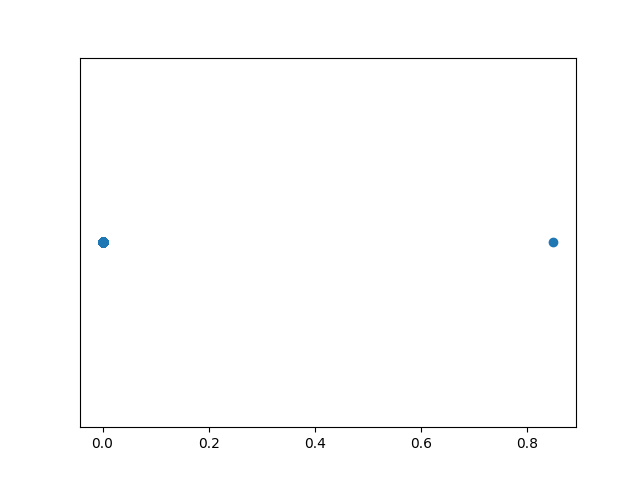
\includegraphics[width=0.5\textwidth]{../figures/eigval_low_rank_sym_no_noise.png}
			\label{fig:eigval_low_rank_without_noise}
		\end{SCfigure}
	
	As shown in figure \ref{fig: eigval_low_rank_without_noise}, only two values are presented in real eigenvalues. Number of ranks $G$ eigenvalues equal the normalization factor $R < 1$ that limits the value range (\ref{eq:eigval_normal}). The rest of $n-G$ eigenvalues take the value $0$. 
	
	The phenomenon of bi-polarized eigenvalue distribution is due to the construction of low-rank RNNs here. If considering the case of having the left connectivity vectors as orthonormal basis for construction of RNNs from (\ref{eq:sym_low_rank}), which is
		\begin{equation} \label{eq:sym_low_rank_eigval}
			J = \frac{1}{n}\sum_{g =1}^{G} l^{(g)} l^{(g)T} = \sum_{g =1}^{G} \frac{1}{n} l^{(g)} l^{(g)T}\, . 
		\end{equation}
	If the rank equals the number of neurons, $G = n$, the formulation of low-rank matrix (\ref{eq:sym_low_rank_eigval}) is at the same time a symmetric full rank matrix with eigenvectors $\left\{l^{(g)}\right\}$ and all eigenvectors correspond to the same eigenvalue $\frac{1}{n}$. Since the eigenvalues are re-scaled by parameter $R < 1$ to enable the stable steady state , the eigenvalues are equal $R$ based on (\ref{eq:eigval_normal}). 
	
	Now, if the rank $G$ is smaller than the number of neurons $n$, the formulation of low-rank RNN (\ref{eq:sym_low_rank_eigval}) can be rewritten as 
		\begin{equation} \label{eq:sym_low_rank_without_noise_eigval}
			J = \sum_{g =1}^{G} \frac{1}{n} l^{(g)} l^{(g)T} + 0 = \sum_{g =1}^{G} \frac{1}{n} l^{(g)} l^{(g)T} + \sum_{g =G}^{n-G} 0 l^{(g)} l^{(g)T} \, .
		\end{equation}
	So, there are $G$ basis vectors that have eigenvalue $\frac{1}{n}$, which is further re-scaled to $R < 1$. The rest of $n-G$ eigenvectors have eigenvalue $0$. This then results the eigenvalue distribution shown in figure \ref{fig:eigval_low_rank_without_noise}. 
	
	We firstly look at the trial-to-trial correlation and except a positive correlation with the feedforward recurrent alignment. When align the inputs to the symmetric recurrent alignment, the inputs have the mean value matched to the eigenvectors of the network. Due to the feedforward recurrent alignment formulation, the alignment scores are the corresponding eigenvalues (\ref{eq:ffrec_equals_eigval}). 
	
	Since there are only two eigenvalues $R$ and $0$ for the rank smaller than number of neurons $G < n$, we assume that there is no continuous correlation but two groups of trial-to-trial correlation values. However, low feedforward recurrent alignment should still correlated with small trail-to-trial correlation and large alignment score with big trial-to-trial correlation. We expect therefore here a discontinuous positive correlation between trial-to-trial correlation and feedforward recurrent alignment. 
%		\begin{SCfigure}[0.9][h]
%			\centering
%			\caption{\textbf{Trial-to-trial correlation against the feedforward recurrent alignment for low-rank symmetric RNNs without noise.} The positive correlation between feedforward recurrent alignment and trial-to-trial correlation is discontinuous due to the number of eigenvalues under low rank. If having rank $G = 1$, only one feedforward recurrent alignment score take the values $R = 0.85$. The rest concentrates at alignment score $0$ with low trial-to-trial correlation. }
%			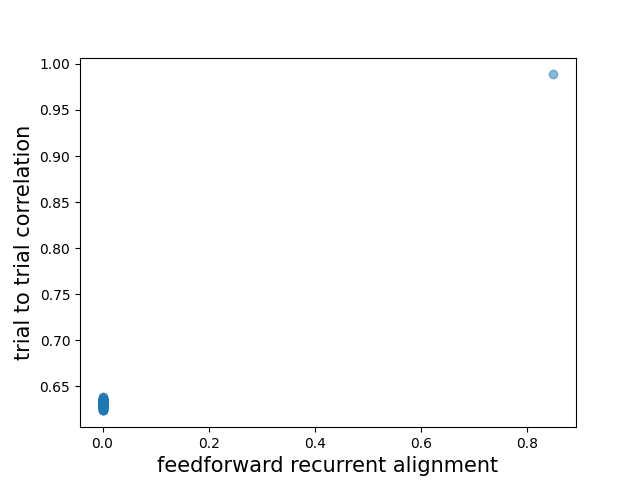
\includegraphics[width=0.5\textwidth]{../figures/low_rank_sym_ttc.png}
%			\label{fig:ttc_low_rank_sym_no_noise}
%		\end{SCfigure}
	
	As the result (figure \ref{fig:ttc_its_low_rank_sym_no_noise}a) show, the trial-to-trial correlation distributes separately in two groups due to the number of eigenvalues. When the feedforward recurrent alignment is low, the trial-to-trial correlation concentrates also at the small number range. The trial-to-trial correlation increases when the feedforward recurrent alignment takes the larger eigenvalue. 
	
%		\begin{SCfigure}[0.9][h]
%			\centering
%			\caption{text}
%			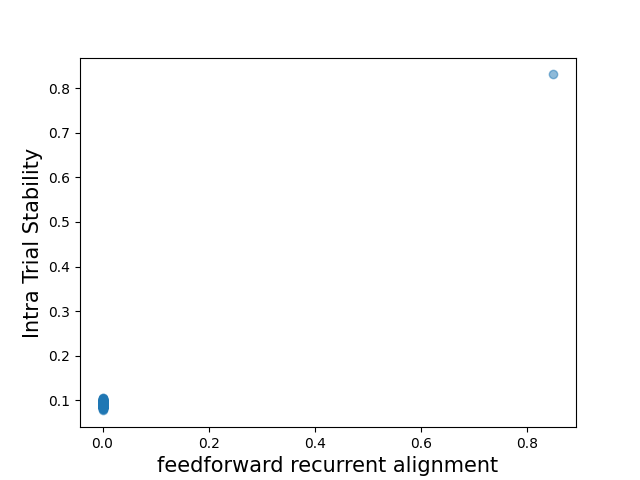
\includegraphics[width=0.5\textwidth]{../figures/its_low_rank_sym_without_noise.png}
%		\end{SCfigure}
%	
		\begin{figure}[H]
			\centering
			\begin{subfigure}[b]{0.45\textwidth}
				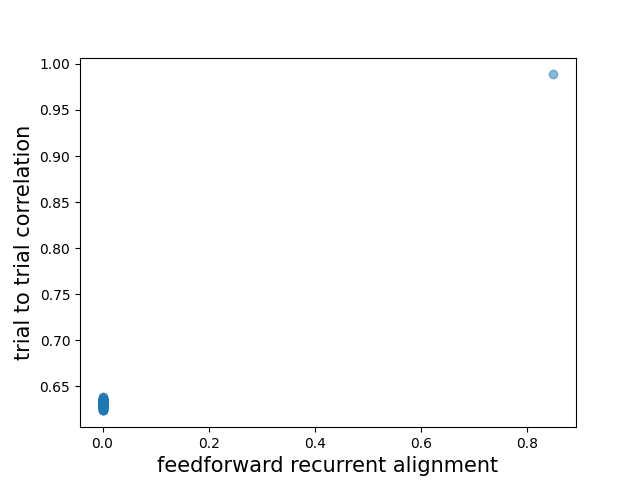
\includegraphics[width=\textwidth]{../figures/low_rank_sym_ttc.png}
				\caption{}
			\end{subfigure}
			\hfill
			\begin{subfigure}[b]{0.45\textwidth}
				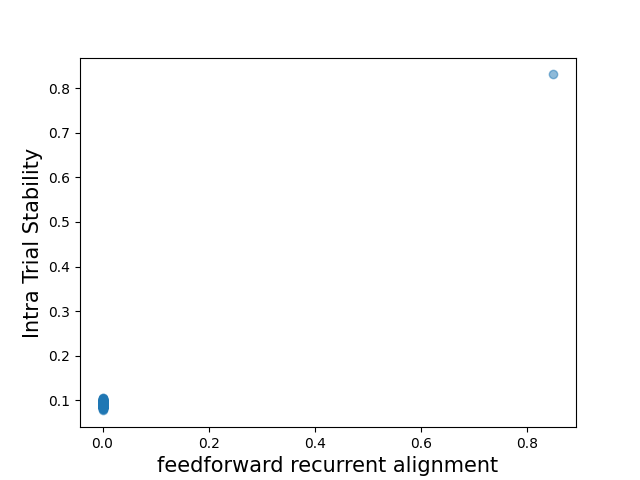
\includegraphics[width=\textwidth]{../figures/its_low_rank_sym_without_noise.png}
				\caption{}
			\end{subfigure}
			\newline
			\begin{subfigure}[b]{0.45\textwidth}
				\includegraphics[width=\textwidth]{../figures/dim_low_rank_sym_without_noise.png}
				\caption{}
			\end{subfigure}
			\hfill
			\begin{subfigure}[b]{0.45\textwidth}
				\includegraphics[width=\textwidth]{../figures/align_to_spont_low_rank_without_noise.png}
				\caption{}
			\end{subfigure}
			\caption{\textbf{Correlation between response properties and feedforward recurrent alignment considering symmetric low-rank RNNs without random noise.} Construct symmetric low-rank RNNs under the assumption of having left connectivity vectors equal right connectivity vectors (\ref{eq:sym_low_rank_eigval}). Rank $G$ is the number of connectivity vectors and significantly smaller than the number of neurons $n$. Here $G = 1$ and $n = 200$. To evaluate the feedforward recurrent alignment hypothesis, the correlations between response properties and the modeled feedforward recurrent alignment score are considered. \\
			\textbf{(a)} Trial-to-trial correlation (y-axis) in correlation with feedforward recurrent alignment score (x-axis).\\
			\textbf{(b)} Intra-trial stability (y-axis) in correlation with feedforward recurrent alignment score (x-axis).\\
			\textbf{(c)} Dimensionality (y-axis) calculated analytically (green dots, (\ref{eq:dim_analytical_sym})) and approximately (blue dots, (\ref{eq:dim_empirical_sym})) in relationship with feedforward recurrent alignment score (x-axis).\\
			\textbf{(d)} Correlation between alignment to spontaneous activity (y-axis) and feedforward recurrent alignment score (x-axis).}
		
%			\caption{\textbf{Trial-to-trial correlation and intra-trial stability in correlation with feedforward recurrent alignment score for low-rank symmetric RNNs.} \textbf{(a)} Trial-to-trial correlation in relationship with feedforward recurrent alignment. \textbf{(b)} Intra-trial stability in relationship with feedforward recurrent alignment.\\ The positive correlation between feedforward recurrent alignment and trial-to-trial correlation \textbf{(a)} or intra-trial stability \textbf{(b)} is discontinuous due to the number of eigenvalues under low rank. If having rank $G = 1$, only one feedforward recurrent alignment score take the value $R = 0.85$, correlating with large trial-to-trial correlation \textbf{(a)} or intra-trial stability \textbf{(b)}. The rest concentrates at alignment score $0$ with low trial-to-trial correlation \textbf{(a)} or low intra-trial stability \textbf{(b)}. }
			\label{fig:ttc_its_low_rank_sym_no_noise}
		\end{figure}
	
	%TODO: Now also consider the other respose properties. 
	% its + reason for not going on with this approach
	Analogous to the trial-to-trial correlation, we suspect the result for intra-trial stability (figure \ref{fig:ttc_its_low_rank_sym_no_noise}b) and alignment to spontaneous activity (figure \ref{fig:ttc_its_low_rank_sym_no_noise}c) also be a discontinuous positive correlation to feedforward recurrent alignment, meanwhile a discontinuous negative correlation for dimensionality (figure \ref{fig:ttc_its_low_rank_sym_no_noise}d). Due to the same reason of existing only two eigenvalues $R$ and $0$, the intra-trial stability value, score of alignment to spontaneous activity distributed, and dimensionality also separately in two groups while keeping the expected correlations with feedforward recurrent alignment. The result (figure \ref{fig:ttc_its_low_rank_sym_no_noise}b) confirmed our assumptions. 
	
%	 Although the positive correlation of feedforward recurrent alignment with both trial-to-trial correlation and intra-trial stability is kept. Since the simple distribution of eigenvalues leads to trivial dynamics between response properties and feedforward recurrent alignment as well as some unwanted effects in dimensionality (Appendix), %TODO:linking
%	 we would rather abandon the formulation of low-rank RNNs for trying modeling feedforward recurrent alignment hypothesis. 
	
	\paragraph{Low-rank RNNs with random noise}
		%The same evaluations considering the response properties are also undertaken for the case when considering the random noise to symmetric low-rank RNNs. 
		\begin{figure}[H]
			\centering
			\begin{subfigure}[b]{0.45\textwidth}
				\centering
				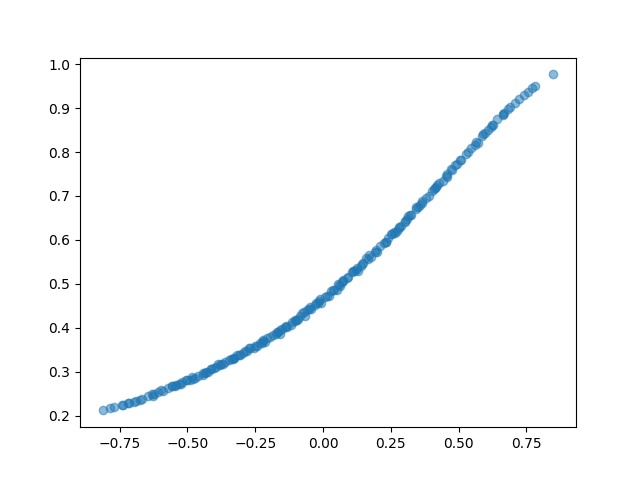
\includegraphics[width=\textwidth]{../figures/ttc_low_rank_sym_with_noise.png}
				\caption{}
			\end{subfigure}
			\hfill
			\begin{subfigure}[b]{0.45\textwidth}
				\centering
				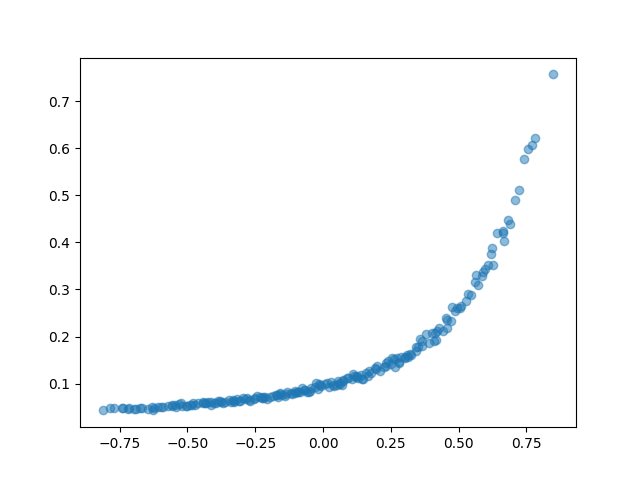
\includegraphics[width=\textwidth]{../figures/its_low_rank_sym_with_noise.png}
				\caption{}
			\end{subfigure}
			\newline
			\begin{subfigure}[b]{0.45\textwidth}
				\centering
				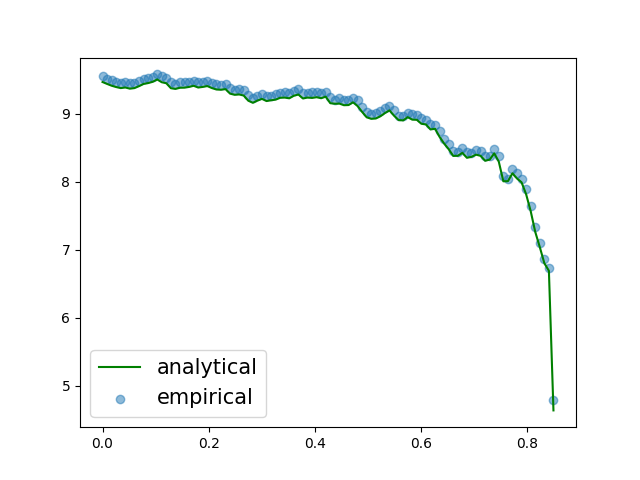
\includegraphics[width=\textwidth]{../figures/dim_low_rank_sym_with_noise.png}
				\caption{}
			\end{subfigure}
			\hfill
			\begin{subfigure}[b]{0.45\textwidth}
				\centering
				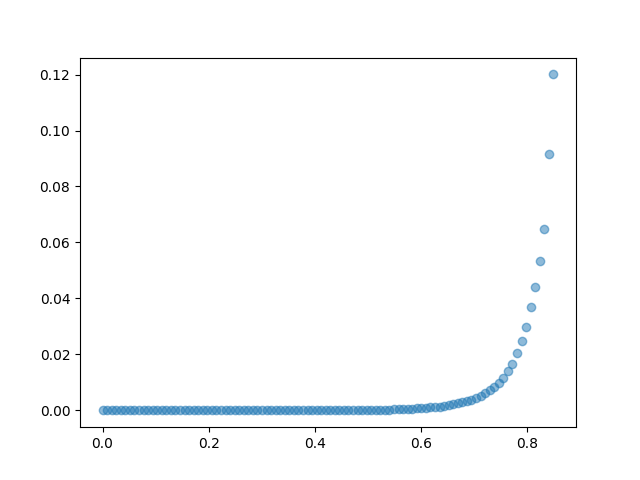
\includegraphics[width=\textwidth]{../figures/spont_align_low_rank_sym_with_noise.png}
				\caption{}
			\end{subfigure}
		\caption{\textbf{Correlation between response properties and feedforward recurrent alignment in symmetric low-rank RNNs with random noise.} Besides the part of a low-rank matrix with rank $G$, RNNs with noise includes an extra part of symmetrized random Gaussian matrix (\ref{eq:low_rank_sym_with_noise}). The rank of low rank part has the rank $G=1$.\\
		\textbf{(a)} Trial-to-trial correlation (y-axis) against feedforward recurrent alignmnet score (x-axis).\\
		\textbf{(b)} Intra-trial stability (y-axis) against feedforward recurrent alignment score (x-axis). \\
		\textbf{(c)} Dimensionality (y-axis) in dependence of feedforward recurrent alignment score (x-axis). Green dots represents the analytical calculation of dimensionality (\ref{eq:dim_analytical_sym}) and blue dots for empirical approximation of dimensionality (\ref{eq:dim_empirical_sym})\\
		 \textbf{(d)} Alignment to spontaneous activity (y-axis) against feedforward recurrent alignment (x-axis).}
	 	\label{fig:result_sym_low_rank_with_noise}
		\end{figure}
%		\begin{figure}[H]
%			\centering
%			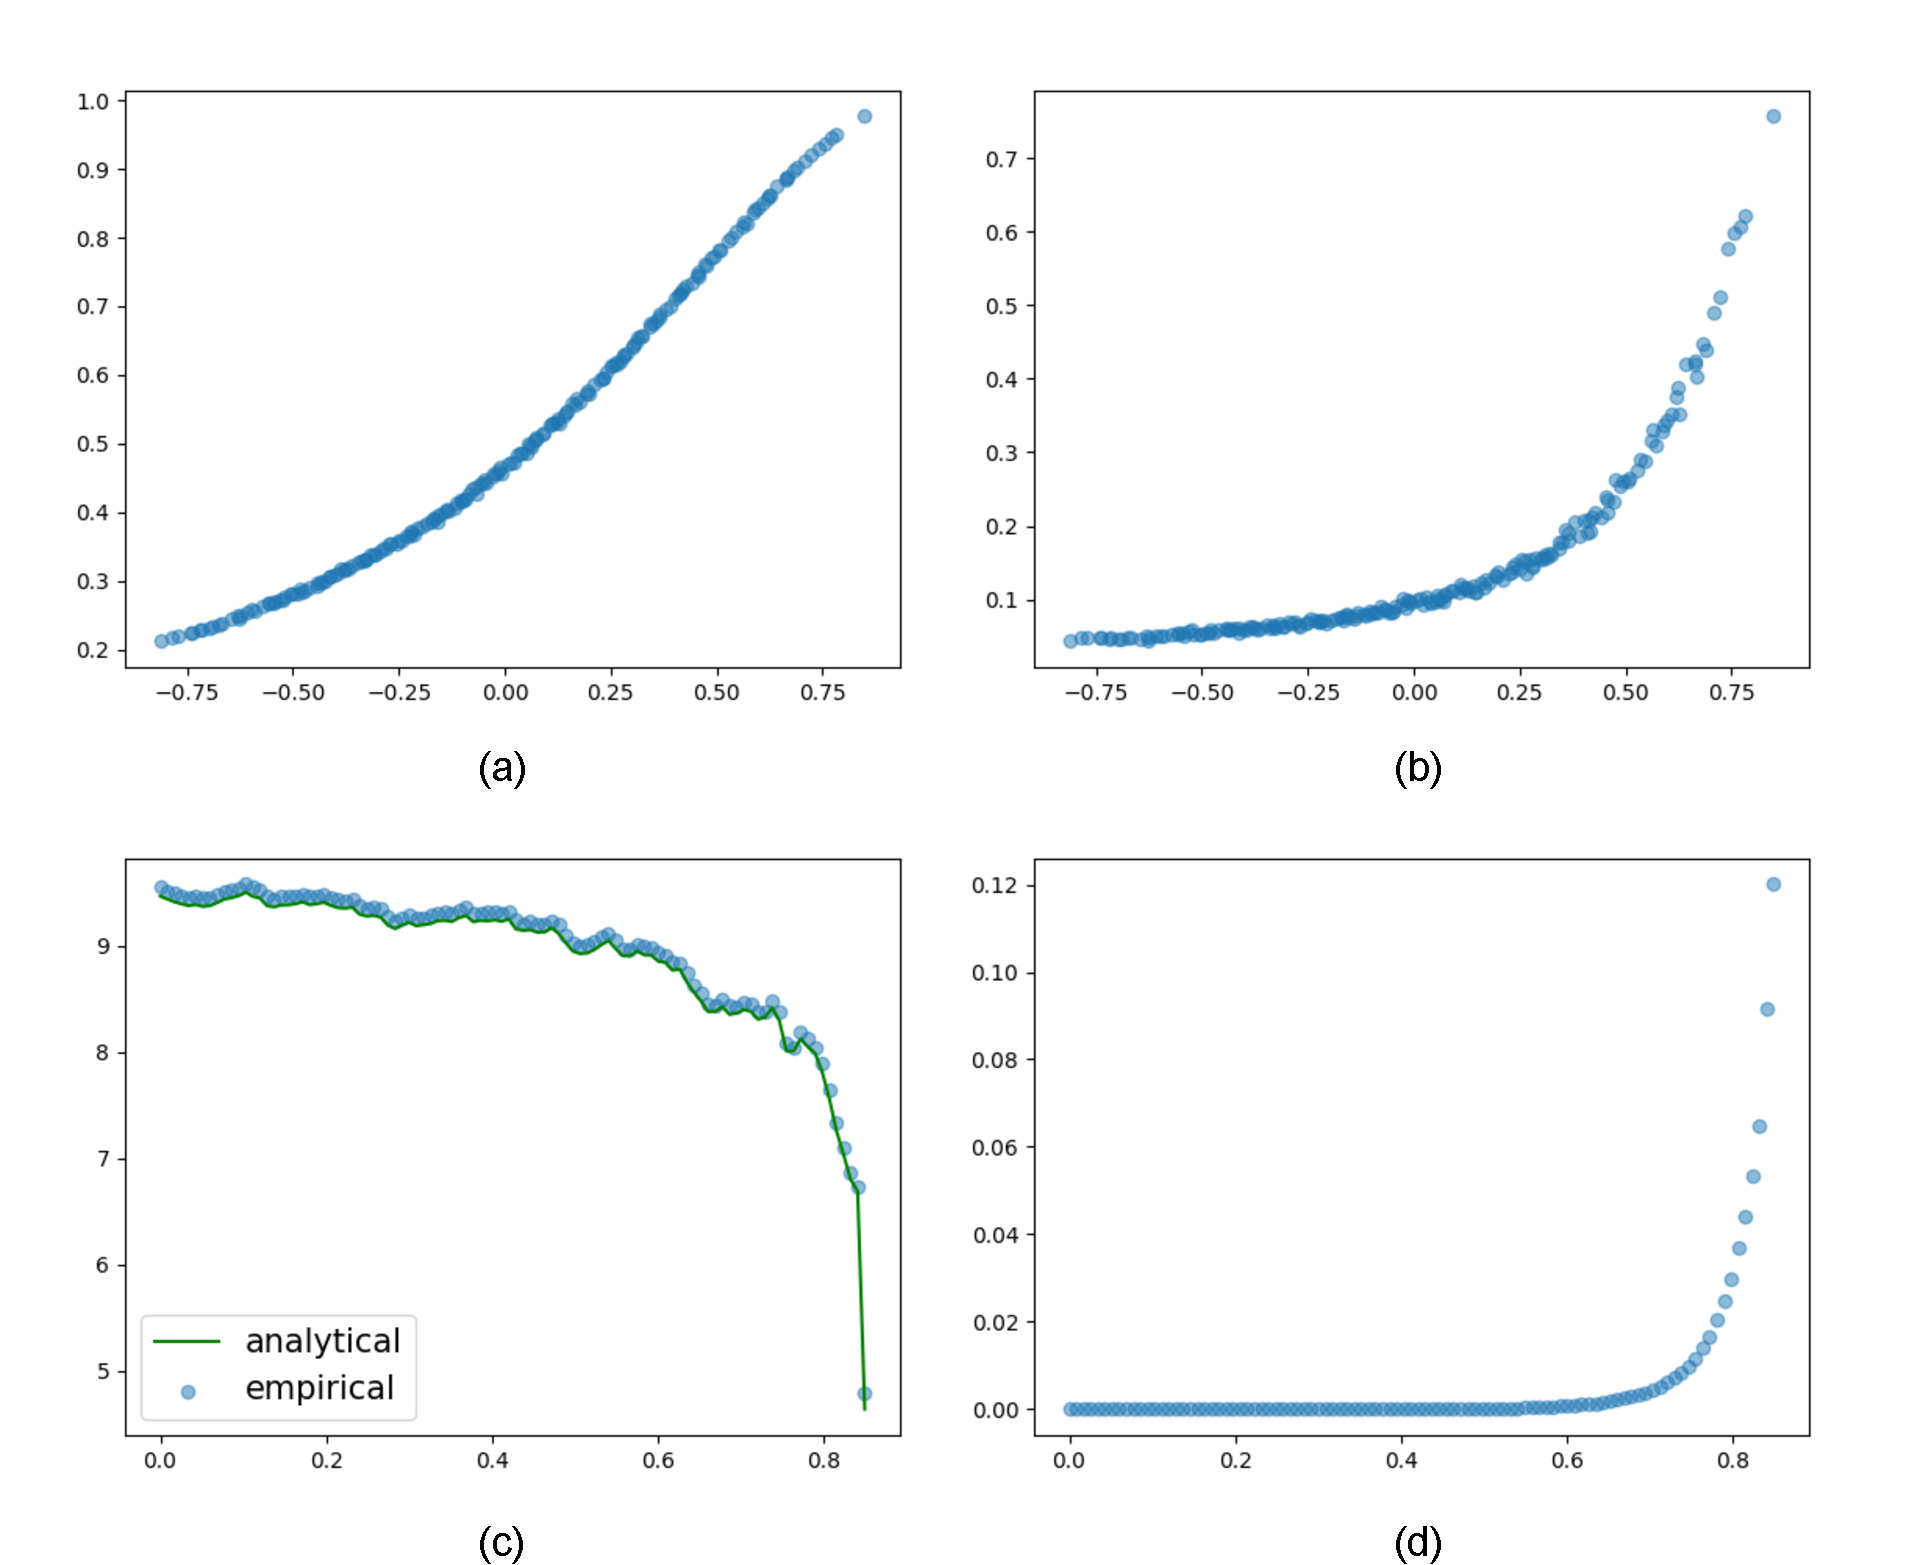
\includegraphics[width=0.8\textwidth]{../figures/low_rank_sym_with_noise.pdf}
%			\caption{\textbf{Correlation between response properties and feedforward recurrent alignment in low-rank RNNs with random noise.} Besides the part of a low-rank matrix with rank $G$, RNNs with noise includes an extra part of symmetrized random Gaussian matrix (\ref{eq:low_rank_sym_with_noise}). The rank of low rank part has the rank $G=1$.\\
%			\textbf{(a)} Trial-to-trial correlation (y-axis) against feedforward recurrent alignmnet score (x-axis). \textbf{(b)} Intra-trial stability (y-axis) against feedforward recurrent alignment score (x-axis). \textbf{(c)} Dimensionality (y-axis) in dependence of feedforward recurrent alignment score (x-axis). \textbf{(d)} Alignment to spontaneous activity (y-axis) against feedforward recurrent alignment (x-axis).}
%		\end{figure}
	
	Low-rank symmetric RNNs with random noise includes extra part of symmetrized Gaussian distributed matrix (\ref{eq:low_rank_with_noise}, section \ref{sec:ffrec_low_rank}). If analog to (\ref{eq:sym_low_rank_eigval}) considering the right connectivity vectors equal the left connectivity vectors, the symmetric low-rank RNNs with random noise can be formulated with a part of symmetric low-rank RNNs and a part of symmetrized Gaussian distributed matrix $J_{\text{rand}}$. 
	\begin{equation} \label{eq:low_rank_sym_with_noise}
		J = \frac{1}{n}\sum_{g =1}^{G} l^{(g)} l^{(g)T} + J_{\text{rand}} \, .
	\end{equation}
	The symmetric random part $J_{\text{rand}}$ should provide more dynamics in the network. 
	
	Since $J_{\text{rand}}$ is a full rank symmetric matrix, the final recurrent network $J$ is also a full rank symmetric matrix in spite of the low-rank symmetric part with rank $G$. Therefore, the correlations between the response properties and feedforward recurrent alignment score are similar to the case of symmetric matrix (figure \ref{fig:ttc_ffrec_sym}, \ref{fig:its_ffrec_sym}, \ref{fig:dim_sym}, and \ref{fig:align_spont_sym}). 
	
	Therefore, the feedforward recurrent alignment hypothesis can be modeled. The expected relationships between feedforward recurrent alignment and response properties (section \ref{sec:results_symmetric}) are fulfilled (figure \ref{fig:result_sym_low_rank_with_noise}). However, the influence of low-rank construction is therefore overwritten by the random noise, which leads to the final dynamics not much different from the case with general random symmetric RNNs. 
	
	\paragraph{Conclusion}
	
	Considering symmetric low-rank RNNs without random noise, the feedforward recurrent alignment keeps the positive correlation to trial-to-trial correlation, intra-trial stability, and alignment to spontaneous activity. Besides, the expected negative correlation between dimensionality and feedforward recurrent alignment is also fulfilled. However, the network construction leads to simple distribution of eigenvalues (\ref{eq:sym_low_rank_eigval}) and in turn also the straightforward distribution of feedforward recurrent alignment score. As a result, only a simple discontinuous correlations of feedforward recurrent alignment to response properties can be observed (figure \ref{fig:ttc_its_low_rank_sym_no_noise}). 
	
	If adding a random noise to disturb the simple dynamics of low-rank RNNs, the final construction (\ref{eq:low_rank_sym_with_noise}) is a full rank symmetric RNN. As a result, the correlations of feedforawrd recurrent alignment to response properties are similar to the results observed in general symmetric RNNs. Although the expected phenomenons are seen, the effect of low-rank RNNs cannot be significantly detected. 
	
	After considering the symmetric low-rank RNNs with and without random noise, although the feedforward recurrent alignment hypothesis can be modeled in both cases. The relationships between feedforward recurrent alignment and response properties meet also the expectations. But either can have significant complex dynamics. Besides, the influence of the rank is also not observable. 
	
	\subsubsection{Different Constructions influence the impact of rank in asymmetric Low-rank RNNs based on response properties}
	
	Asymmetric low-rank RNNs can have more complex dynamics than symmetric low-rank RNNs. Section \ref{sec:ffrec_low_rank} also introduces the construction of asymmetric low-rank RNNs with or without random noise. Generally, if taking the set of left connectivity vectors different from the set of right connectivity vectors, asymmetric matrices can be formulated (\ref{eq:low_rank_RNN_without_noise}), (\ref{eq:low_rank_with_noise}). 
	
	% Choose symmetrized method from privious results. 
	Since asymmetric low-rank RNNs are only a certain case of asymmetric RNNs with specific constructions, they also have the problem of complex eigenvectors and eigenvalues when modeling the feedforward recurrent alignment hypothesis. Therefore, from the previous results with general asymmetric RNNs, we choose the modification of aligning inputs to symmetrized RNN because of the overall best performance among all considered modifications (section \ref{sec:asymmetric_results}).
	
	\paragraph{Low-rank RNNs without random noise}
	
	Asymmetric low-rank RNNs without random noise consist of non-equal left and right connectivity vectors, which are mutually orthogonal (figure \ref{fig:low_rank_RNN_without_noise}) (\ref{eq:low_rank_RNN_without_noise}). 
		\begin{figure}[H]
			\centering
			\begin{subfigure}[b]{0.3\textwidth}
				\centering
				\includegraphics[width=\textwidth]{../figures/eigval_distribution_asym_low_rank_without_noise.png}
				\caption{rank$=1$}
			\end{subfigure}
			\begin{subfigure}[b]{0.3\textwidth}
				\centering
				\includegraphics[width=\textwidth]{../figures/eigval_distribution_asym_low_rank_without_noise(2).png}
				\caption{rank$=5$}
			\end{subfigure}
			\begin{subfigure}[b]{0.3\textwidth}
				\centering
				\includegraphics[width=\textwidth]{../figures/eigval_distribution_asym_low_rank_without_noise(3).png}
				\caption{rank$=10$}
			\end{subfigure}
			\caption{\textbf{Eigenvalue distribution in dependence of rank by asymmetric low-rank RNNs without random noise.} The asymmetric low-rank RNNs without random noise is constructed by mutually orthogonal non-equal left and right connectivity vectors. The number of vector pairs $G$ also determines the rank of the interaction matrix, which should be significantly smaller than the number of neurons $G \ll n$ (\ref{eq:low_rank_RNN_without_noise}). The rank $G$ can influence the distribution of eigenvalues for asymmetric low-rank RNNs in complex plane. x-axis for real part and y-axis for imaginary part. \textbf{(a)} Eigenvalue distribution under rank $G=1$. \textbf{(b)} Eigenvalue distribution under rank $G=5$. \textbf{(c)} Eigenvalue distribution under rank $G=10$. }
			\label{fig:eigval_distribution_asym_low_rank_without_noise}
		\end{figure}
	
	For symmetric low-rank RNNs without random noise, as long as the rank $G$ is significantly smaller than the number of neurons $n$ as defined, the distribution of eigenvalues separating into two groups (figure \ref{fig:eigval_low_rank_without_noise}) keeps the unchanged. While for asymmetric low-rank RNNs without random noise, the influence of rank $G$ is more significant (figure \ref{fig:eigval_distribution_asym_low_rank_without_noise}). 
	
	The construction of asymmetric low-rank RNNs without random noise can be understood as $G$ pairs of connectivity vectors are represented, while the rest of $n-G$ pairs are suppressed (\ref{eq:low_rank_RNN_without_noise}), formally written out with
		\begin{equation} \label{eq:asym_low_rank_RNNs_without_noise_eigval}
			J = \frac{1}{n} \sum_{g=1}^{G} l^{(g)} r^{(g)T} = \sum_{g=1}^{G} \frac{1}{n} l^{(g)} r^{(g)T} + \sum_{g=1}^{n-G} 0 l^{(g)} r^{(g)T} \, .
		\end{equation}
	Therefore, exactly $G$ number of eigenvalues do not concentrate at $0$ but the rest $n-G$ eigenvalues are (figure \ref{fig:eigval_distribution_asym_low_rank_without_noise}). Since the mathematical construction for asymmetric low-rank RNNs is not a eigendecomposition (\ref{eq:asym_low_rank_RNNs_without_noise_eigval}), the eigenvalues after re-scaling by normalization parameter $R$ (method section \ref{sec:ffrec_low_rank}) do not exactly have magnitude $R$ as at symmetric low-rank RNNs (\ref{eq:sym_low_rank_without_noise_eigval}).	
	
		\begin{figure}[H]
			\centering
			\begin{subfigure}[b]{0.3\textwidth}
				\includegraphics[width=\textwidth]{../figures/ttc_asym_low_rank_without_noise_rank=1.png}
				\caption{rank$=1$}
			\end{subfigure}
			\begin{subfigure}[b]{0.3\textwidth}
				\includegraphics[width=\textwidth]{../figures/ttc_asym_low_rank_without_noise_rank=5.png}
				\caption{rank$=5$}
			\end{subfigure}
			\begin{subfigure}[b]{0.3\textwidth}
				\includegraphics[width=\textwidth]{../figures/ttc_asym_low_rank_without_noise_rank=10.png}
				\caption{rank$=10$}
			\end{subfigure} 
			\caption{\textbf{Relationship of trial-to-trial correlation and feedforward recurrent alignment in dependence of rank by asymmetric low-rank RNNs without random noise.} The rank $G$ in asymmetric low-rank RNNs (\ref{eq:asym_low_rank_RNNs_without_noise_eigval}) influence the distribution thus also the distribution of trial-to-trial correlation. Rank $G$ is significantly smaller than the number of neurons $n$ by definition. $n=200$. Illustrate the correlation between feedforward recurrent alignment and trial-to-trial correlation under varied ranks. \textbf{(a)} correlation under rank $G=1$. \textbf{(b)} correlation under rank $G=5$. \textbf{(c)} correlation under rank $G=10$.} 
			\label{fig:ttc_asym_low_rank_RNN_without_noise}
		\end{figure}
	% Suspect that symmetrization lead to reflection and double set/number of eigenvalues. 
	% Erwartung
	We expect that the distribution of the correlation between feedforward recurrent alignment and trial-to-trial correlation will be determined by the eigenvalue distribution (figure \ref{fig:eigval_distribution_asym_low_rank_without_noise}) under different ranks. Besides, a positive correlation between feedforward recurrent alignment and trial-to-trial correlation should be maintained independent of the change of rank.
	
	% Results
	As expected, the rank influence the eigenvalue distribution and thus also the correlation distribution between feedforward recurrent alignment and trial-to-trial correlation. However, the positive correlation is not kept over the range of feedforward recurrent alignment. In fact, it can be observed that the distribution is almost identical in the negative and positive range of feedfroward recurrent alignment. The number of dots in each half-range also exactly equal the number of range, or the number of non-zero eigenvalues in (figure \ref{fig:eigval_distribution_asym_low_rank_without_noise}). Therefore, there are now doubled number of non-zero feedforward recurrent alignment scores as expected. 
		
	% Reaseon for results.
	Our assumption is that the reflection and duplication could due to the symmetrization of asymmetric low-rank RNNs with simple construction of only applying connectivity vectors. With the symmetrization, a part of reflected network also contributes to eigenvalue expression and therefore increase the number of presented feedforward recurrent alignment. Symmetrization of (\ref{eq:asym_low_rank_RNNs_without_noise_eigval}) leads to
		\begin{equation} \label{eq:asym_low_rank_without_noise_symmetrization}
			J_{\text{sym}} = \frac{J + J^T}{2} = \frac{1}{2n} \left( \sum_{g=1}^{G} l^{(g)} r^{(g)T} + \sum_{g=1}^{G} r^{(g)} l^{(g)T}\right) = \frac{1}{2n} \sum_{g=1}^{G} l^{(g)} r^{(g)T} + \frac{1}{2n} \sum_{g=1}^{G} r^{(g)} l^{(g)T} \, .
		\end{equation}
	The second part of (\ref{eq:asym_low_rank_without_noise_symmetrization}) is presumed to be the reason for the distribution in negative range of feedforward recurrent alignment in figure \ref{fig:ttc_asym_low_rank_RNN_without_noise}. The construction (\ref{eq:asym_low_rank_without_noise_symmetrization}) doubles the network in two sub networks separately by unexpressed connectivity vectors. Each sub-network spread over the negative or the positive range of feedforward recurrent alignment. A positive correlation between feedforward recurrent alignment and trial-to-trial correlation can be observed in each half range. But there is therefore no positive correlation overall. 
	
	Thus, the modeling of feedforward recurrent alignment hypothesis in this case cannot fulfill the phenomenon over the whole range of alignment between inputs and recurrent network. 
	% TODO: Appendix the result of intra-trial stability, dimensionality, and alignment to spontaneous activity? 
	
	\paragraph{Low-rank RNNs with random noise}
	% General introduction of low-rank RNNs.
	Above without random noise, the simple construction dose not performance well with the modification of alignment to symmetrized recurrent network. Now, we add a Gaussian distributed asymmetric random part to the simple construction. As a result, the asymmetric recurrent network is composed of a low-rank part from connectivity vectors and a part of full rank random noise (eq. (\ref{eq:low_rank_with_noise}) and method section \ref{sec:ffrec_low_rank}). The final recurrent network is therefore full rank asymmetric. 
	
	% Expectations. 
	If the feedforward recurrent alignment hypothesis can be modeled in the asymmetric low-rank RNNs with random noise, positive correlations between feedforward recurrent alignment score and trial-to-trial correlation, intra-trial stability, and alignment to spontaneous activity are expected. Moreover, dimensionality should be negatively correlated with feedforward recurrent alignment. On the basis of observations from symmetric low-rank RNNs with random noise (figure \ref{fig:result_sym_low_rank_with_noise}), the results can be similar to the case with general asymmetric full rank RNNs (section \ref{sec:asym_ffrec_response}). In other words, the dynamics of low-rank can be suppressed by full rank noise dynamics.  
	%However, on the other hand, the random noise could cover the effect from low-rank part. 
	
	% Analysis of results.
	The results (figure \ref{fig:result_asym_low_rank_with_noise}) confirmed our expectations of correlations between response properties and feedforward recurrent alignment that the correlations have high similarity to the results we got from general asymmetric RNNs. Under the strong effect of full rank random noise, the difference cased by low-rank part is not significant (compare blue and orange dots in figure \ref{fig:result_asym_low_rank_with_noise}). The results in section \ref{sec:asymmetric_results} indicates that the dispersion increases with larger proportion of asymmetry in RNNs. Since the final construction consists only of asymmetric networks, the dispersion is large especially at dimensionality. 
	% In spite of the suppression effect of full rank random noise, the influence can still be slightly observed, especially in the correlation between feedforward recurrent alignment and alignment to spontaneous activity (figure \ref{fig:result_asym_low_rank_with_noise}d). Low rank (blue dots in figure \ref{fig:result_asym_low_rank_with_noise}d) leads to a stronger dispersion of the correlation than a "higher" rank (orange dots in figure \ref{fig:result_asym_low_rank_with_noise}d).
	% Results.
		\vspace{-0.2cm}
		\begin{figure}[H]
			\centering
			\begin{subfigure}[b]{0.45\textwidth}
				\centering
				\includegraphics[width=\textwidth]{../figures/ttc_asym_low_rank_with_noise_rank=1_5.png}
				\caption{}
			\end{subfigure}
			\hfill
			\begin{subfigure}[b]{0.45\textwidth}
				\centering
				\includegraphics[width=\textwidth]{../figures/its_asym_low_rank_with_noise_rank=1_5.png}
				\caption{}
			\end{subfigure}
			\newline
			\begin{subfigure}[b]{0.45\textwidth}
				\centering
				\includegraphics[width=\textwidth]{../figures/dim_asym_low_rank_with_noise_rank=1_5.png}
				\caption{}
			\end{subfigure}
			\hfill
			\begin{subfigure}[b]{0.45\textwidth}
				\centering
				\includegraphics[width=\textwidth]{../figures/align_spont_asym_low_rank_with_noise_rank=1_5.png}
				\caption{}
			\end{subfigure}
		\caption{\textbf{Correlations between feedforward recurrent alignment and selected response properties for asymmetric low-rank RNNs with random noise.} Additional to the low-rank part constructed only by left and right connectivity vectors, a Gaussian distributed full rank asymmetric random noise is included in the network dynamic (\ref{eq:low_rank_with_noise}). Due to the full rank random noise, the results has large similarity to results from general asymmetric RNNs. Two different ranks are taken to assess the influence of ranks to correlations. The rank $G$ should be significantly smaller than the number of neurons $n$. \\
		With $n = 200$, comparing ranks $G = 1$ in blue dots with $G=5$ in orange:\\
		\textbf{(a)} Correlation between feedforward recurrent alignment (x-axis) and trial-to-trial correlation (y-axis). \\
		\textbf{(b)} Correlation between feedforward recurrent alignment (x-axis) and intra-trial stability (y-axis). \\
		\textbf{(c)} Dimensionality (y-axis) calculated analytically (lines, blue line for $G=1$ and orange line for $G=5$) and empirically in correlation with feedforward recurrent alignment (x-axis).\\
		\textbf{(d)} Alignment of evoked patterns to spontaneous activity (y-axis) in relationship with feedforward recurrent alignment (x-axis).}
		\label{fig:result_asym_low_rank_with_noise}
		\end{figure}
 
	% Reason for the dispersion? Only with rank = 10 has small dispersion. Other ranks has the same degree of dispersion...
	
	\paragraph{Conclusion}
	We explored the modeling of feedforward recurrent alignment in asymmetric low-rank RNNs. Two types of constructions are taken into account: 1) single part of non-equal left and right connectivity vectors and 2) with additional full rank random noise (defined in method section \ref{sec:ffrec_low_rank}). 
	
	The simple construction without random noise has eigenvalue distribution depending on the rank. Keeping the rank significantly smaller than the number of neurons, the number of non-zero eigenvalues equal the rank. Thus, the number of non-zero feedforward recurrent alignment score also depends on the rank. Due to the modification of aligning inputs to symmetrized RNNs for calculation of feedforward recurrent alignment score, the correlation between alignment score and trial-to-trial correlation is separated into two sub-groups. As a result, although in each sub-region the positive correlation between alignment score and trial-to-trial correlation is kept, there is no global positive correlation over the total range. 
	
	Adding the full rank random noise can avoid the effect of doubling caused by symmetrization. The expected positive correlations between feedforward recurrent alignment and trail-to-trial correlation, intra-trial stability, and alignment to spontaneous activity are kept. Large dispersion is caused by the total asymmetry of RNNs. In spite of large dispersion, the negative correlation between dimensionality and feedforward recurrent alignment can be observed. However, expression of low-rank connections is suppressed by the full rank random noise, such that there is no significant difference between RNNs with various ranks. 
	
	\clearpage
	\subsection{White Noise Evoked Activity Can Help to Approximate Dominant Activity Direction in Response Space for Unknown Asymmetric Recurrent Networks}
	% TODO: Die Quelle kann noch bisschen spezifisch sein wenn ich noch mehr davon weiß. 
	% Background/Problem.
	Normally during experimental procedures, the complete recurrent network structure of the laboratory animal keeps unknown. Therefore, even if the feedforward recurrent alignment hypothesis can be theoretically underpinned well in both symmetric and asymmetric recurrent networks (section \ref{sec:results_symmetric} and section \ref{sec:asym_ffrec_response}), the hypothesis cannot be well undertaken in experimental environments. 
	
	% Goal
	Our goal here is to achieve a theoretical framework for the feedforwar recurrent alignment that is compatible experimentally without knowing the exact recurrent network structure. 
	% Spontanoues activity.
	
	Motivated by some predictions from a series of theoretical frameworks \cite{mulholland2023selective, marre2009reliable} that the matching between inputs and spontaneous activity can lead to more reliable evoked responses and more efficient transmission across cortical networks, we consider the idea of generating spontaneous-like activity pattern for alignment as an approximation of the original recurrent network. 
	
	% Use white noise to approximate spontaneous activity. 
	To generate spontaneous-like activity patterns, experimentally methods with white noise is suggested by the lab of H.Mulholland.  %TODO: Is this correct? Reference of Video/Postabstracts. 
	Therefore, we model the white noise and its evoked activity theoretically for construction of modified feedforward recurrent alignment score with principal components of white noise evoked activity pattern. Evaluation of our framework covers mainly four perspectives of response properties, namely trial-to-trial correlation, intra-trial stability, dimensionality, and alignment of evoked activity to spontaneous activity (method section \ref{sec:white_noise_approx_ffrec}). 
	
	\subsubsection{Positive Monotonic Correlation between Feedforward Recurrent Alignment Score and Eigenvalues of White Noise Evoked Activity Pattern}
	
	% Reason for monotony (review from the method caption). + expactations + results.
	Feedforward recurrent alignment score (\ref{sec:white_noise_approx_ffrec}) should reflect how well the input is aligned with the dominant direction of response space for recurrent network. Since the original recurrent network is unknown, we apply the white noise evoked activity pattern for approximation of the alignment. Therefore, aligning the input to principal components of white noise evoked activity pattern instead of the original recurrent network. 
	
	A positive monotony correlation between feedforward recurrent and variance ratio of aligned white noise evoked activity pattern is essential for guaranteeing the functionality of feedforward recurrent alignment score. Due to the selective response amplification (\ref{eq:response_amplification}), the dominant variance ratio (aka. eigenvalues of covariance matrix) of white noise evoked pattern should determine the response. Thus, the feedforward recurrent alignment should have a high value when aligning to the corresponding principal components of dominant variance ratio, indicating that the evoked response would be reliable. The monotony guarantees that the alignment to dominant principal components is the only source for increase of the feedforward recurrent alignment score. 
	
	% was wir machen wollen: ffrec nun sollte funktionieren. Also wenn es groß ist, sollte die resposnes properties gut sein --> durch alignment to white noise evoked act. kann man auch die development von response properties klären. 
		\begin{SCfigure}[0.9][h] 
			\centering
			\caption{0}
			\includegraphics[width=0.5\textwidth]{imagefile}
			\label{}
		\end{SCfigure}
	
	\subsubsection{Evaluation of Approximation with white noise through Response Properties}
	
	\paragraph{Trial-to-trial Correlation}
	
	\paragraph{Intra-trial Stability}
	
	\paragraph{Dimensionality}
	
	\paragraph{Alignment to Spontaneous Activity}
	
	\paragraph{Conclusion}
	
\end{document}